\documentclass[a4paper,12pt]{article}
\usepackage{amsmath}
\usepackage{graphicx}
\usepackage{hyperref}
\usepackage{siunitx}
\title{Guida alla Creazione di un Grafico a Dispersione con Google Sheets}
\author{Insegnante di Fisica}

\begin{document}

\maketitle

\section{Introduzione}
In questa sezione, impareremo come creare un grafico a dispersione utilizzando Google Sheets. Seguendo passo per passo, vedremo come inserire i dati, creare il grafico, personalizzarlo con titolo e etichette, e aggiungere una linea di tendenza. Infine, vedremo come mostrare due grafici contemporaneamente.

\section{Creazione del Documento}
\begin{enumerate}
    \item Apri Google Sheets e crea un nuovo foglio di calcolo.
    
\begin{figure}[h!]
    \centering
    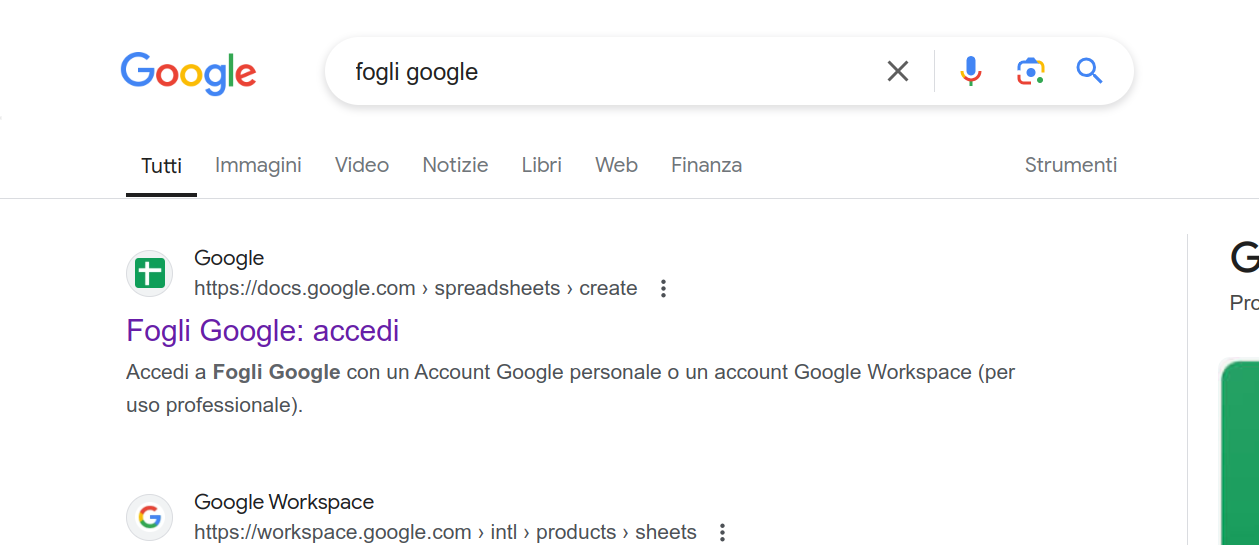
\includegraphics[width=\linewidth]{path_to_image/creadoc.png} 
    \caption{Creazione del documento in Google Sheets}
\end{figure}    
    
    \item Rinomina il foglio in modo appropriato, ad esempio, \textit{Esperimento di Fisica}.
    \begin{figure}[h!]
    \centering
    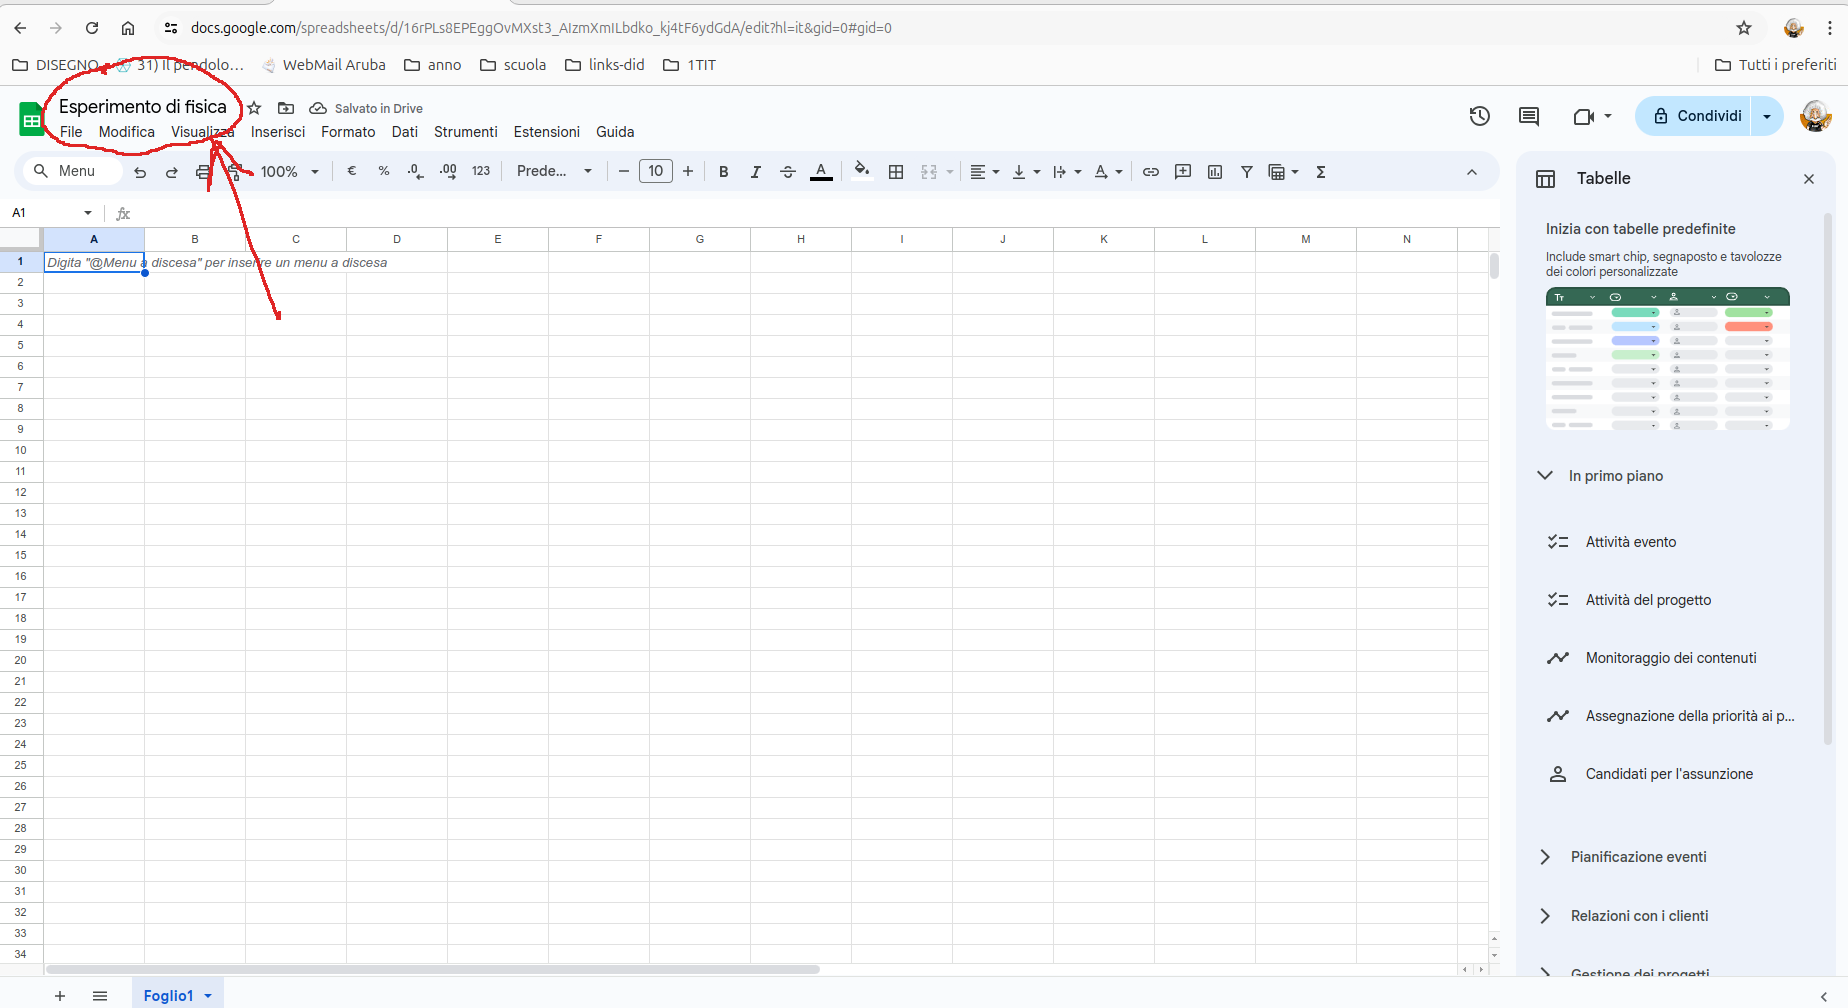
\includegraphics[width=\linewidth]{path_to_image/rinomina.png} 
    \caption{Rinomina il  documento in Google Sheets}
\end{figure} 
\end{enumerate}


\section{Inserimento dei Dati}
\begin{enumerate}
    \item Inserisci i dati nelle colonne A e B. Ad esempio, nella colonna A metti i valori della variabile indipendente (ad esempio, tempo in secondi), e nella colonna B i valori della variabile dipendente (ad esempio, distanza in metri).
    \item Digita i dati manualmente, facendo clic su una cella e digitando il valore. Premi \textbf{Invio} per passare alla cella sottostante.
    \item Esempio di dati:
    \begin{center}
    \begin{tabular}{|c|c|}
    \hline
    Tempo (s) & Distanza (m) \\
    \hline
    1 & 1,2 \\
    2 & 2,5 \\
    3 & 3,1 \\
    4 & 4,0 \\
    5 & 5,3 \\
    \hline
    \end{tabular}
    \end{center}
\end{enumerate}
    \begin{figure}[h!]
    \centering
    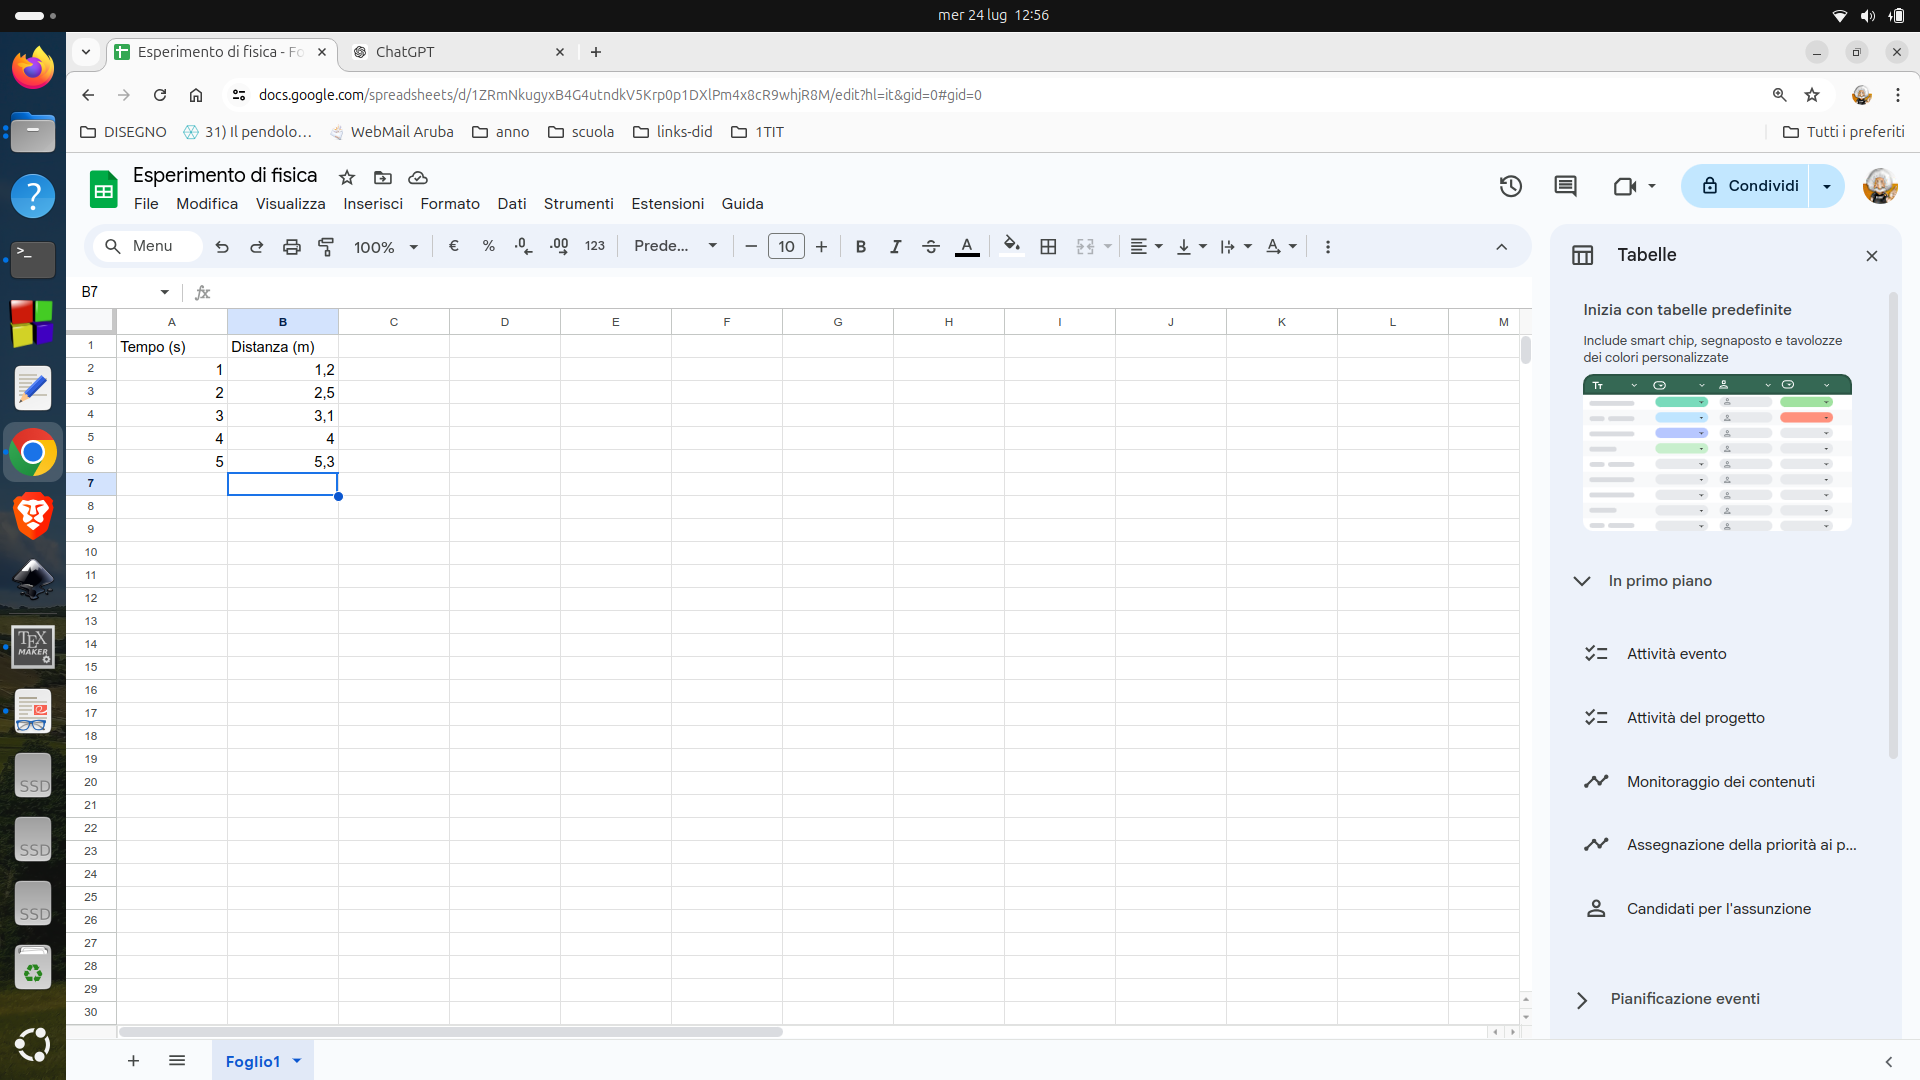
\includegraphics[width=\linewidth]{path_to_image/dati.png} 
    \caption{Inserimento dei dati.}
\end{figure} 

Da notare che Google Sheets (``fogli di calcolo'', in italiano) utilizza le virgole per i numeri decimali (esattamente come facciamo noi). Altri programmi (e calcolatrici) invece, usano i puntini. Vi accorgete che il foglio di calcolo considera effettivamente scritte come 1,2 come numeri, perché li allinea a destra nella cella.


\section{Creazione del Grafico a Dispersione}
\begin{enumerate}
    \item Seleziona i dati inseriti nelle colonne A e B. Puoi farlo cliccando e trascinando il mouse dall'angolo superiore sinistro (A1) all'angolo inferiore destro (B5) dei tuoi dati.
     \begin{figure}[h!]
    \centering
    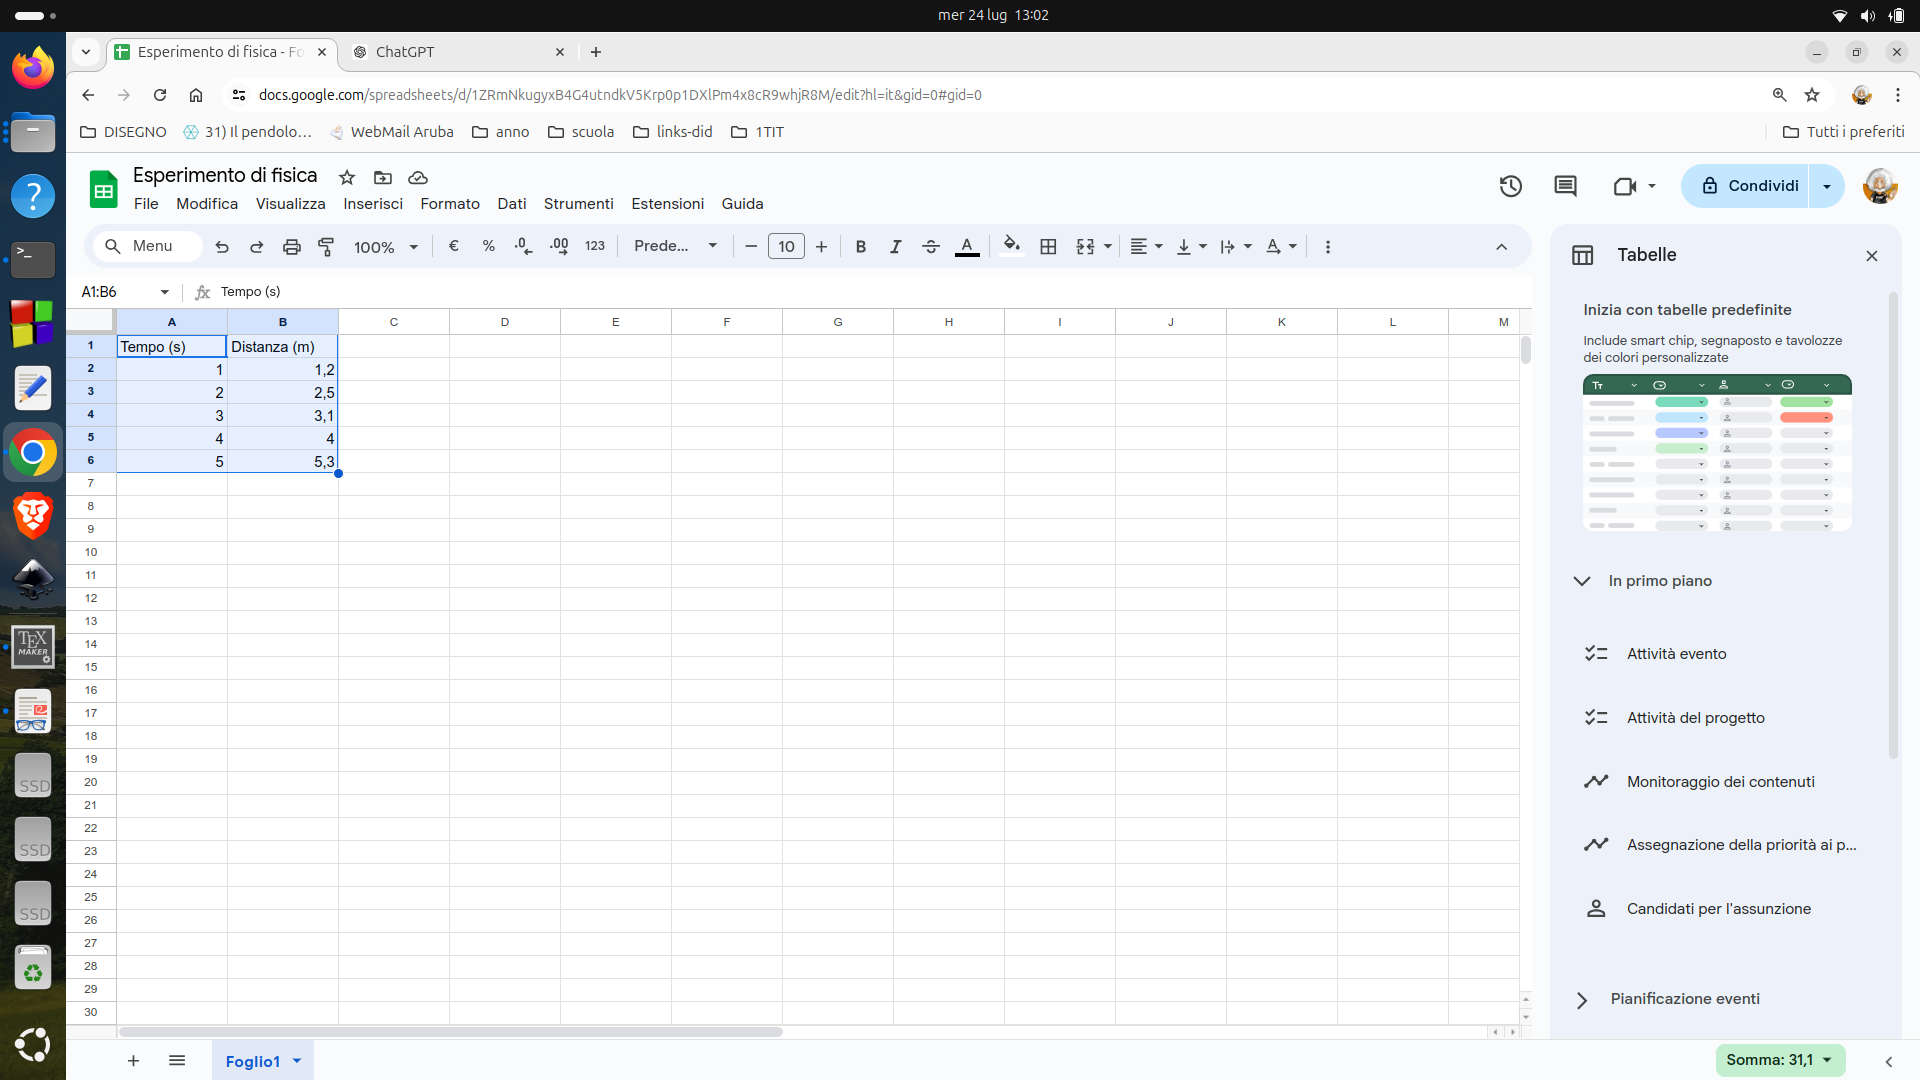
\includegraphics[width=\linewidth]{path_to_image/selezione.png} 
    \caption{Seleziome dei dati.}
\end{figure} 
    
    
    \item Vai su \textbf{Inserisci} nel menu e seleziona \textbf{Grafico}.
    
        \begin{figure}[h!]
    \centering
    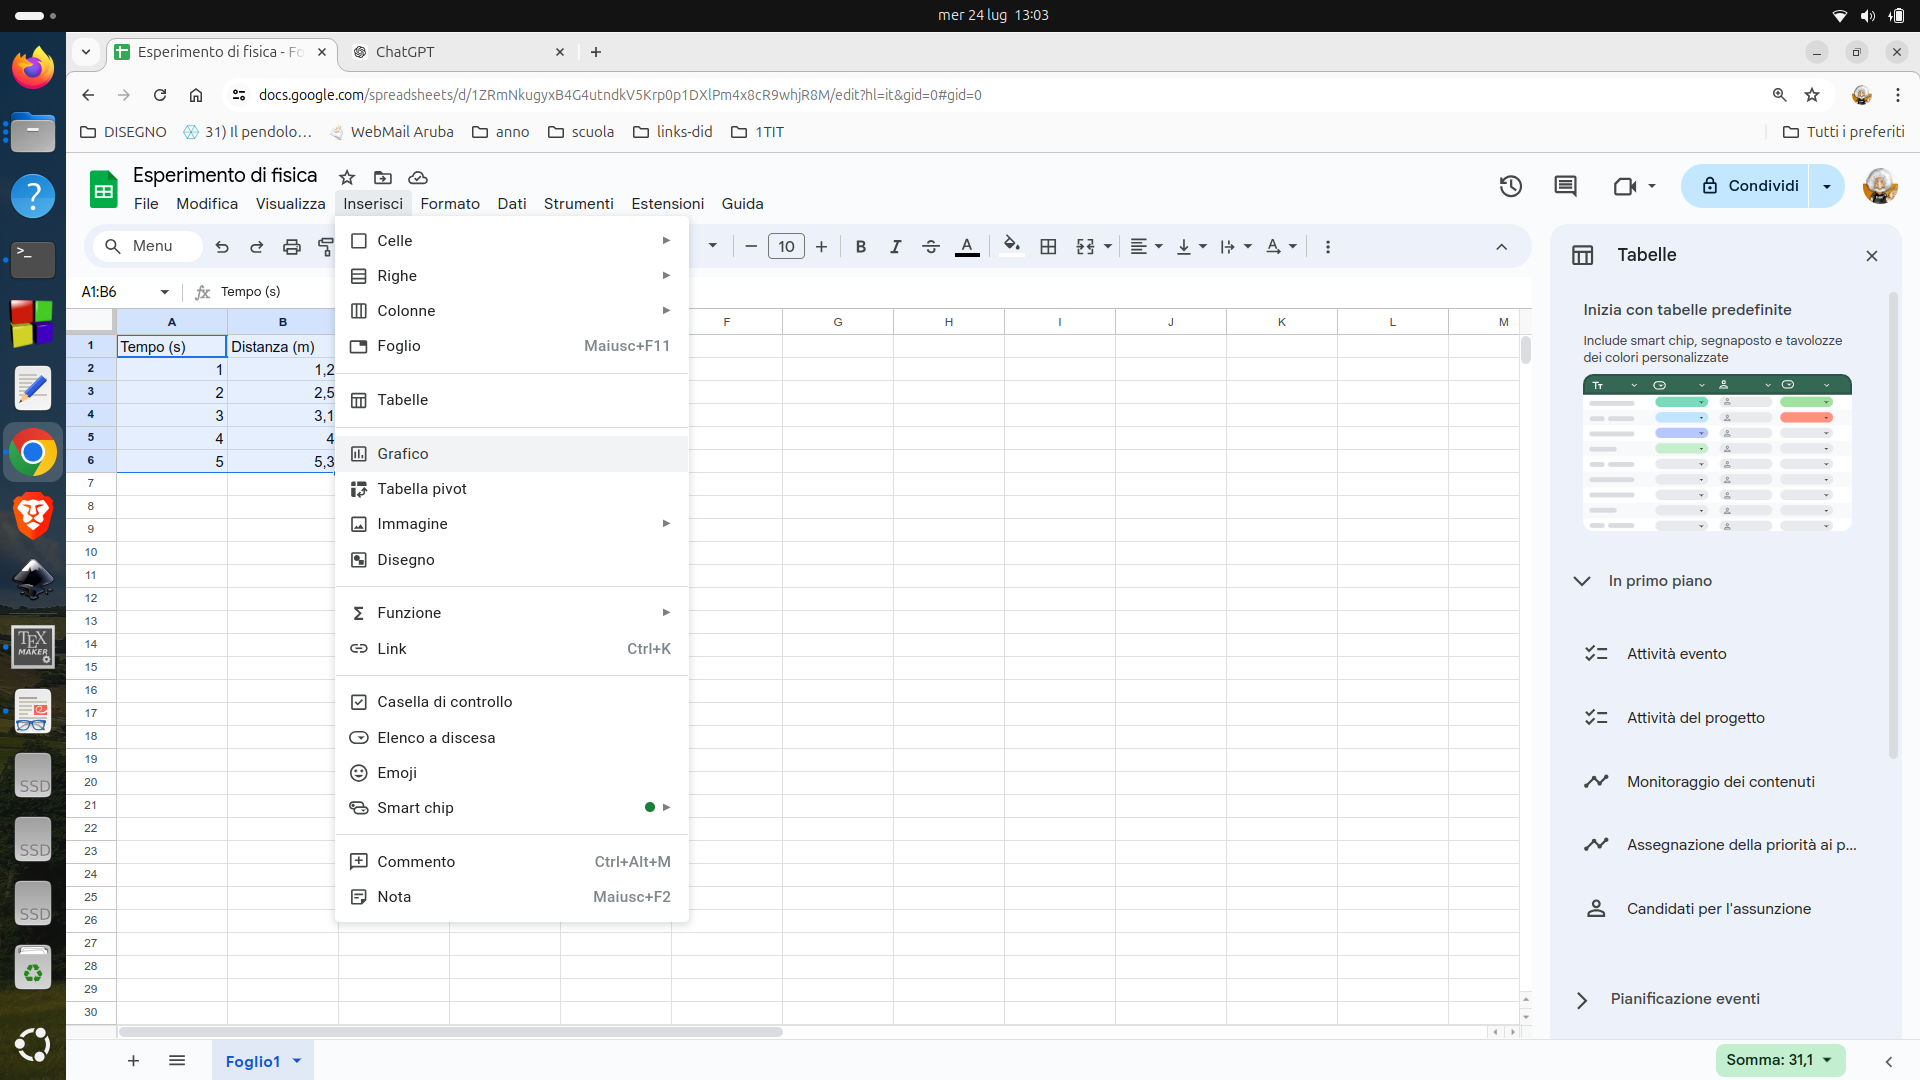
\includegraphics[width=\linewidth]{path_to_image/inseriscigrafico.png} 
    \caption{Inserimento del grafico.}
\end{figure}  
    
    
    
    \item Nella finestra delle opzioni del grafico, seleziona \textbf{Grafico a dispersione} dal menu a tendina \textbf{Tipo di grafico}.
    
            \begin{figure}[h!]
    \centering
    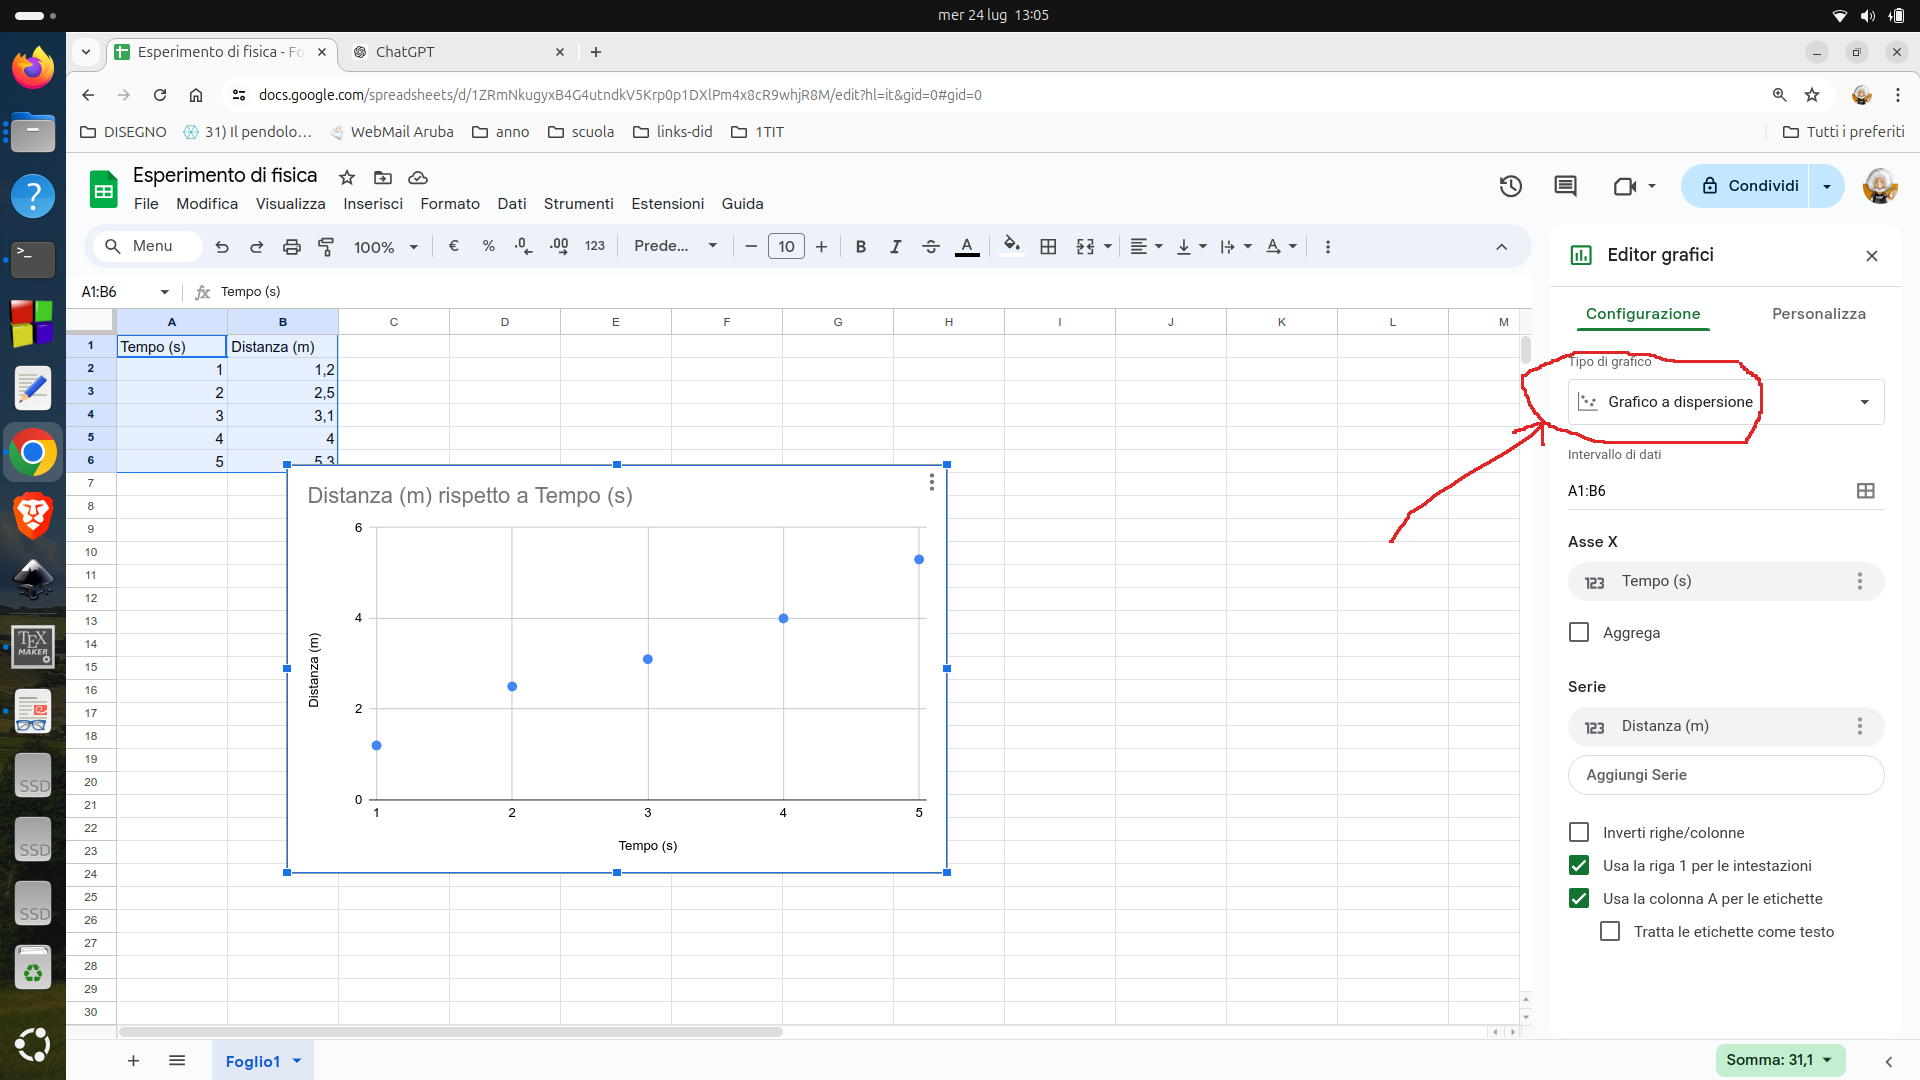
\includegraphics[width=\linewidth]{path_to_image/dispersione.png} 
    \caption{Grafico a dispersione.}
\end{figure} 
\end{enumerate}



\section{Personalizzazione del Grafico}
\begin{enumerate}
    \item Per personalizzare il grafico, devi aprire la finestra di modifica (a destra). Se non è già visibile, clicca i tre puntini sul grafico e scegli \textbf{modifica}. Se non vedi i tre puntini, clicca su un'area bianca sul grafico (non sul foglio di calcolo, proprio sul grafico):
    
    \begin{figure}[h!]
    \centering
    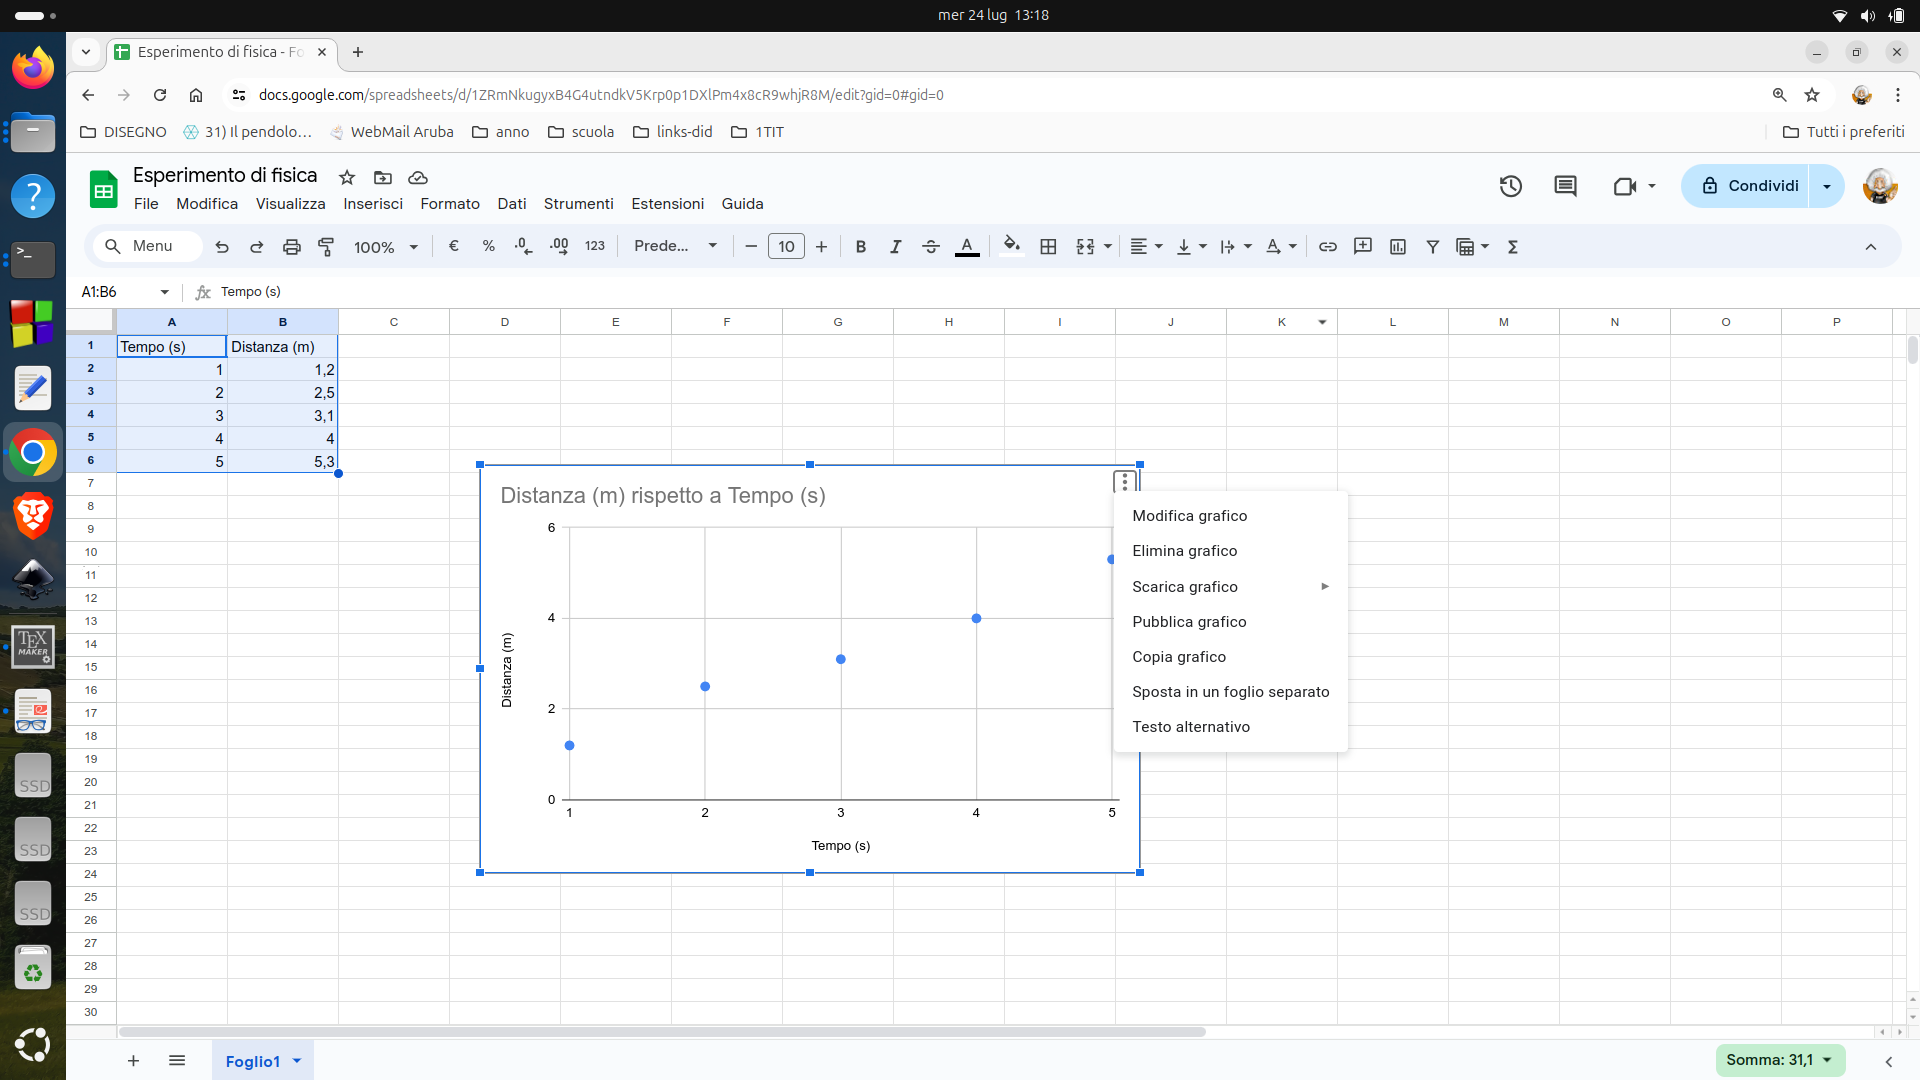
\includegraphics[width=\linewidth]{path_to_image/modifica.png} 
    \caption{Modifica del grafico.}
\end{figure} 
    
    \item Clicca sulla scheda \textbf{personalizza} (figura \ref{fig:personalizza})
    \begin{figure}[h!]
    \centering
    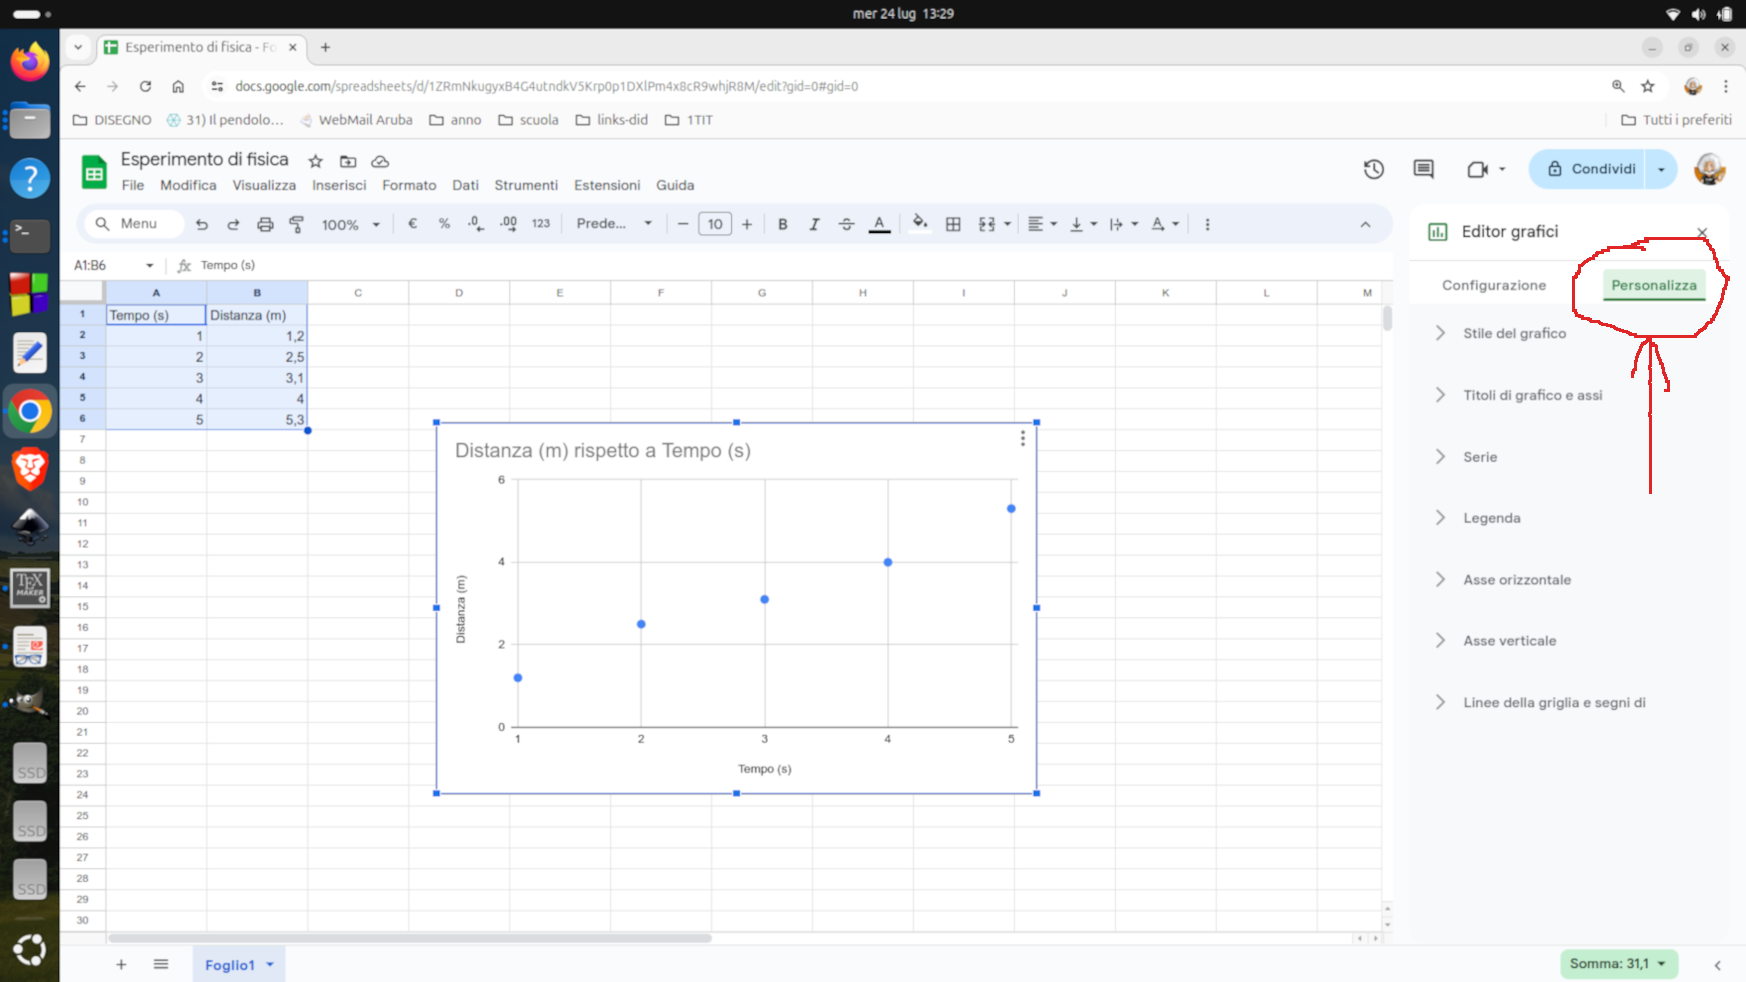
\includegraphics[width=\linewidth]{path_to_image/personalizza.png} 
    \caption{Scheda \textbf{Scheda personalizza.}}
    \label{fig:personalizza}
\end{figure} 
    
    
    \item Aggiungi il titolo del grafico: ad esempio, \textit{Relazione tra Tempo e Distanza}: espandendo il sottomenu \textbf{Titolo di grafico e assi} figura \ref{fig:titolo}:
    
 \begin{figure}[h!]
    \centering
    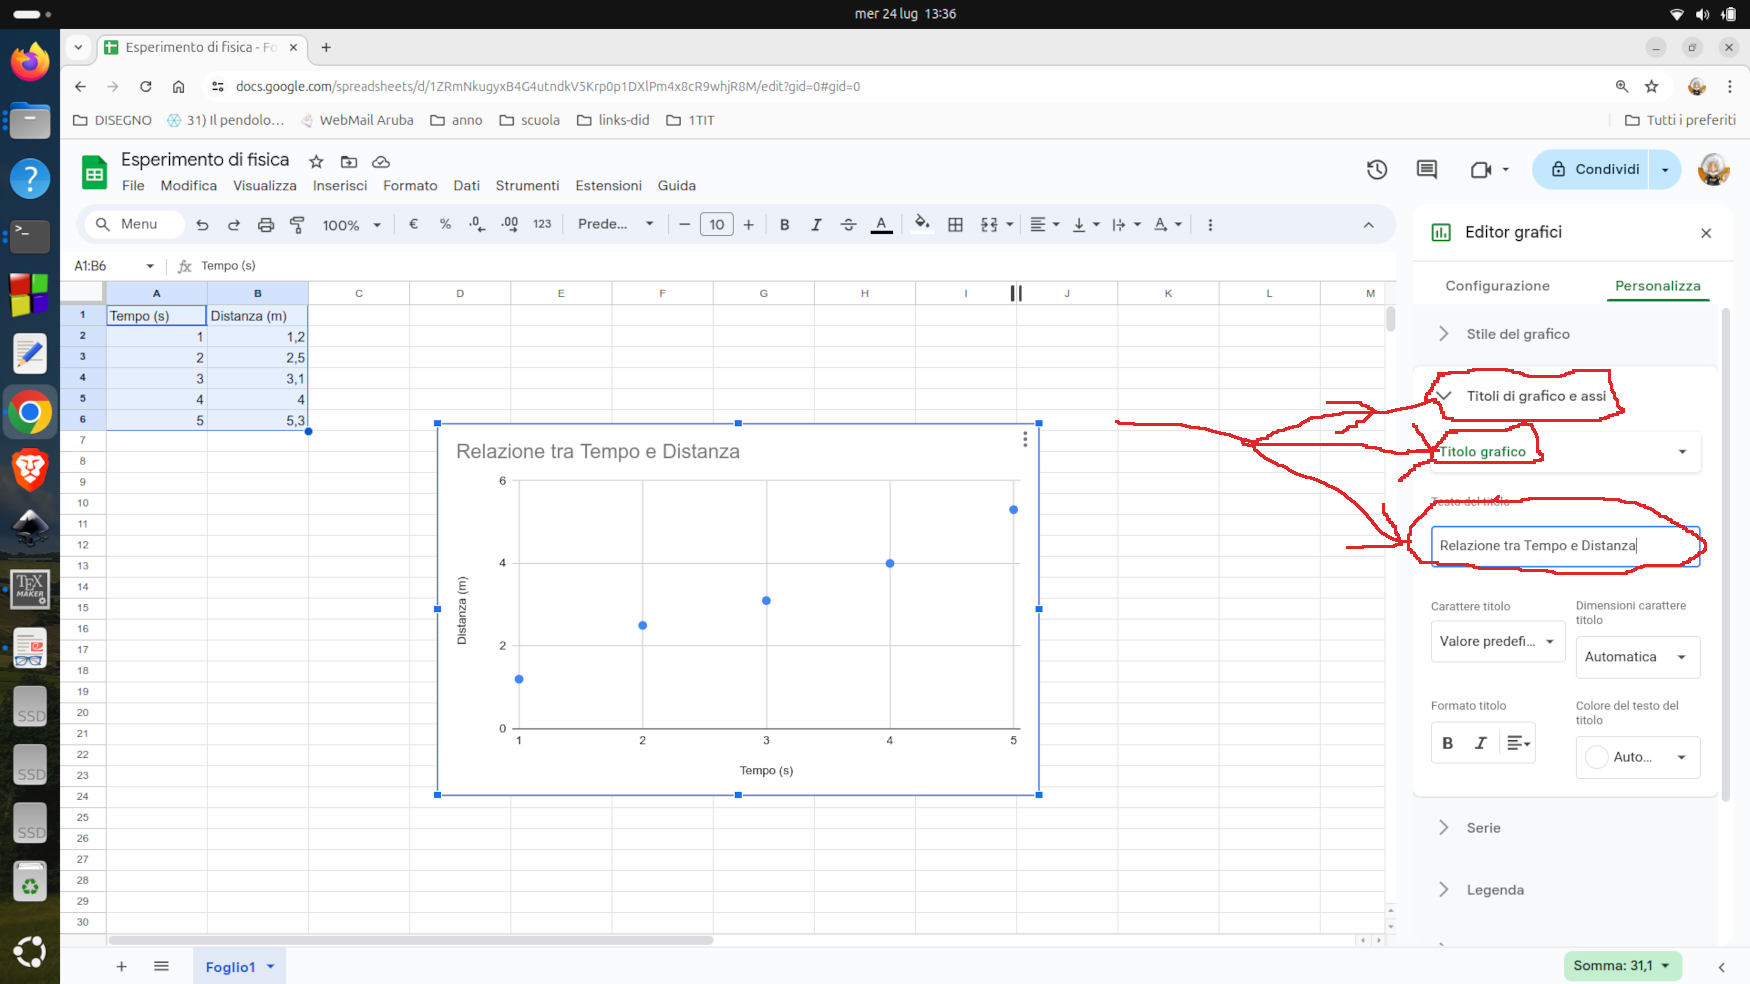
\includegraphics[width=\linewidth]{path_to_image/titolo.png} 
    \caption{Scheda \textbf{Modifica del titolo.}}
    \label{fig:titolo}
\end{figure} 
    
    \item Aggiungi le etichette agli assi. Seleziona dal menu a tendina \textbf{Titolo asse orizzontale: } (figura \ref{fig:sceltax})
        \begin{figure}[h!]
    \centering
    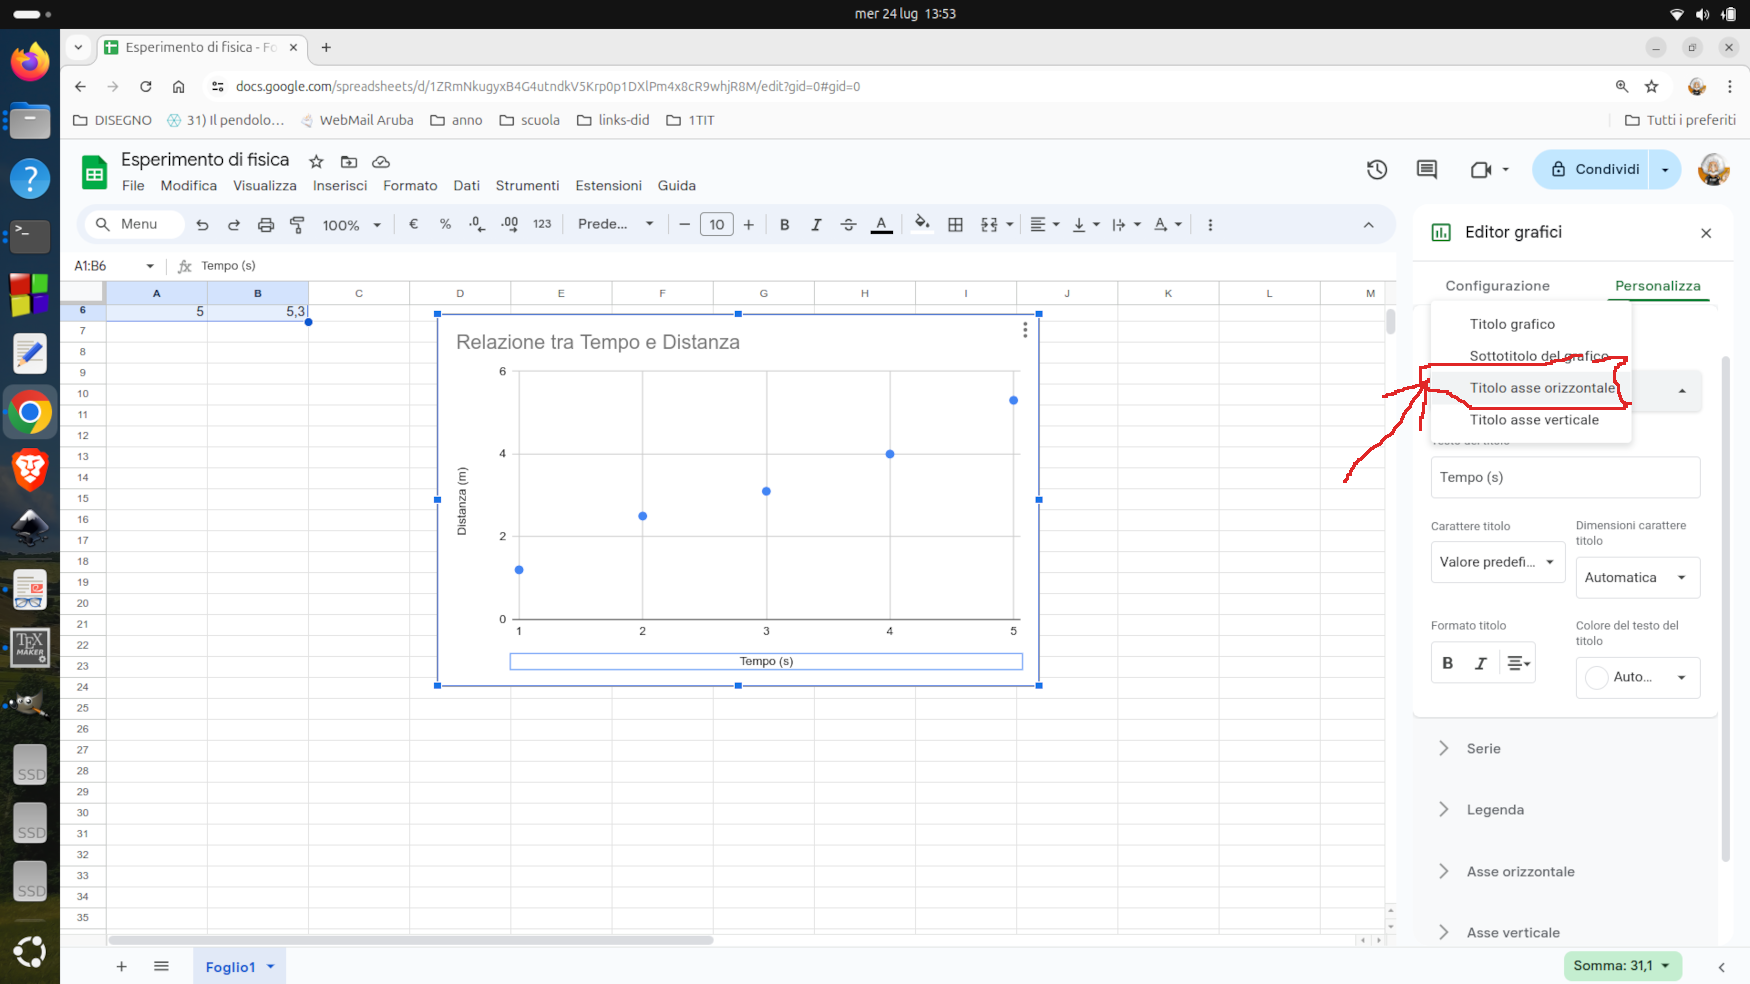
\includegraphics[width=\linewidth]{path_to_image/sceltax.png} 
    \caption{Scelta menu per il titolo dell'asse orizzontale.}
    \label{fig:sceltax}
\end{figure}  
        
        
        \item Imposta il titolo per l'asse X: \textit{Tempo (s)} (figura \ref{fig:titolox})
        
       \begin{figure}[h!]
    \centering
    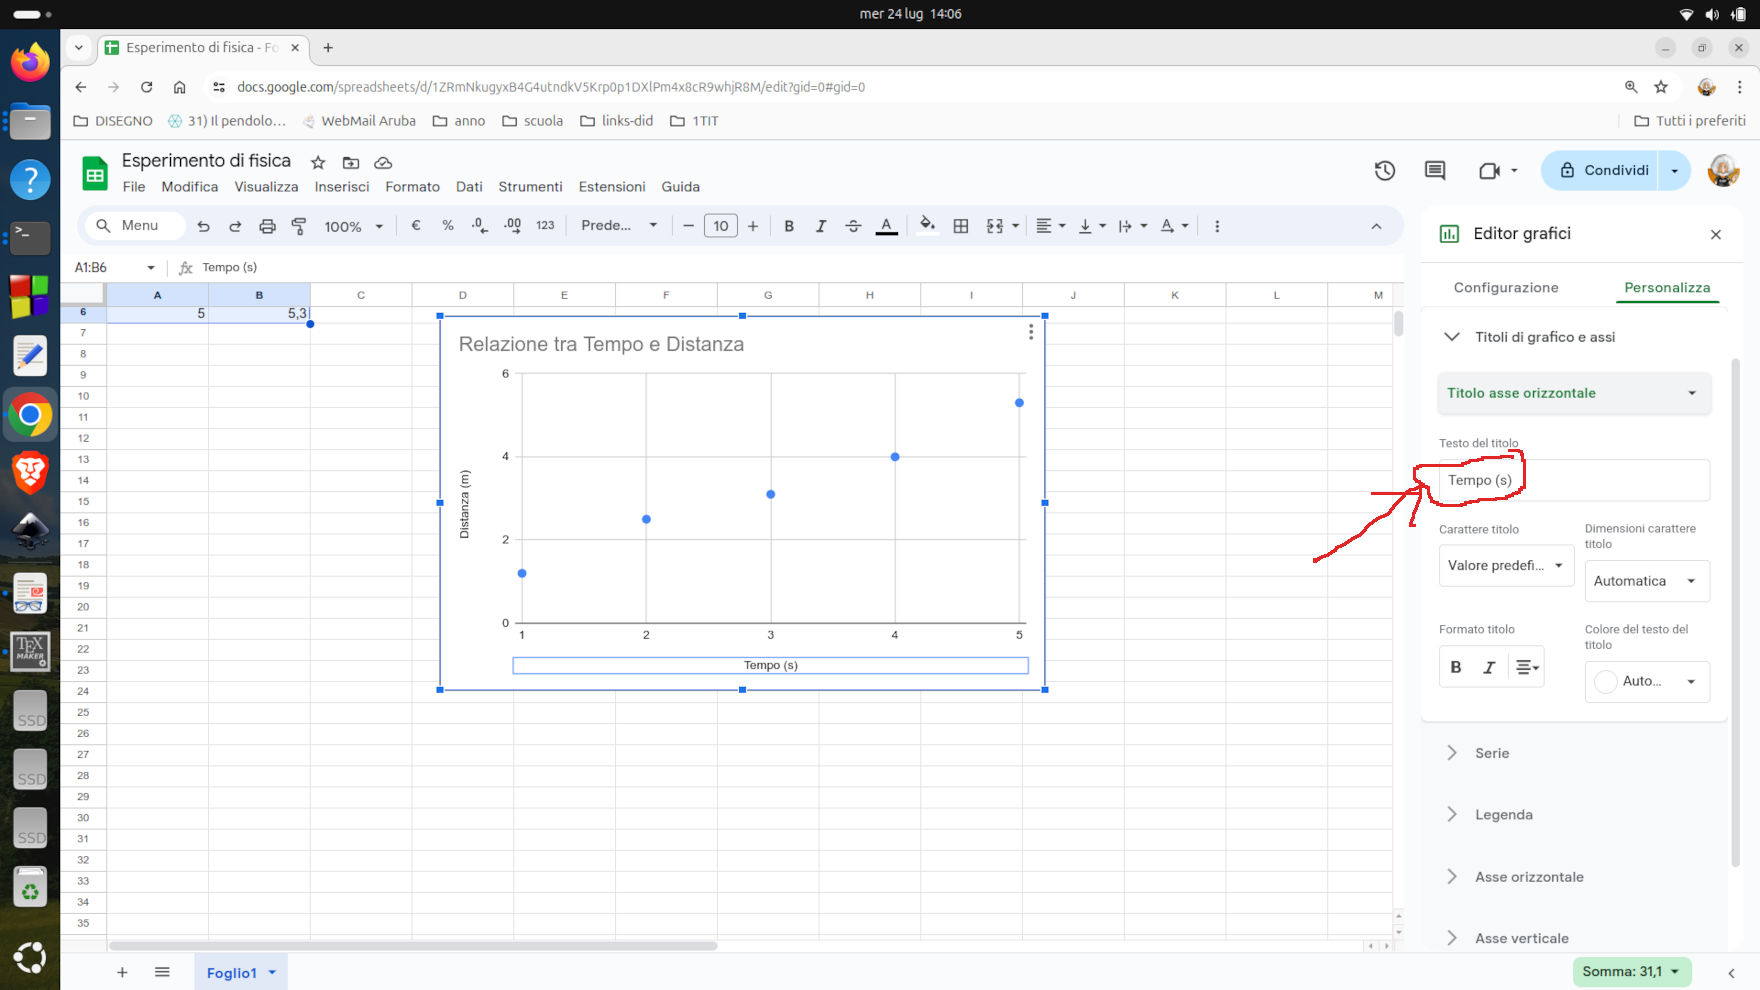
\includegraphics[width=\linewidth]{path_to_image/titolox.png} 
    \caption{Scelta del titolo per l'asse x}
    \label{fig:titolox}
\end{figure} 



    \item Seleziona dal menu a tendina \textbf{Titolo asse verticale: } (figura \ref{fig:sceltay})  (figura \ref{fig:sceltay})  
    \begin{figure}[h!]
    \centering
    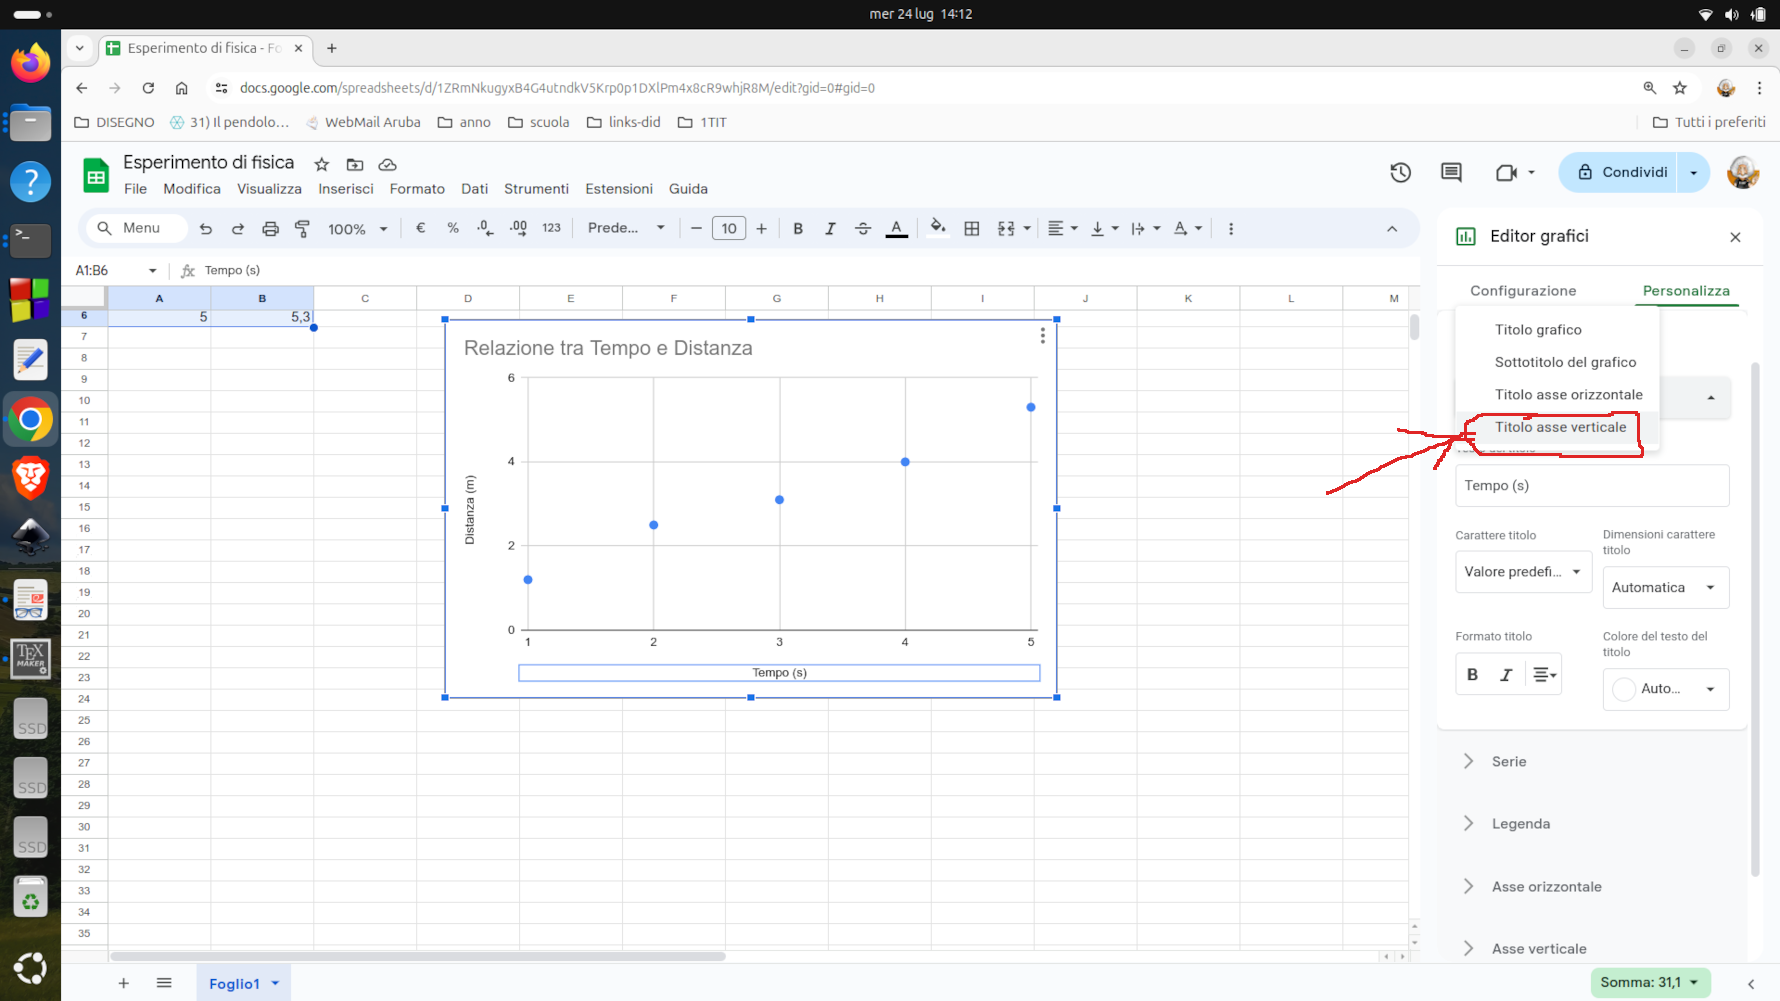
\includegraphics[width=\linewidth]{path_to_image/sceltay.png} 
    \caption{Scelta menu per l'asse verticale.}
    \label{fig:sceltay}
\end{figure}  



        \item Imposta un titolo per l'asse  Y: \textit{Distanza (m)} (figura \ref{fig:titoloy})
        
    
\begin{figure}[h!]
    \centering
    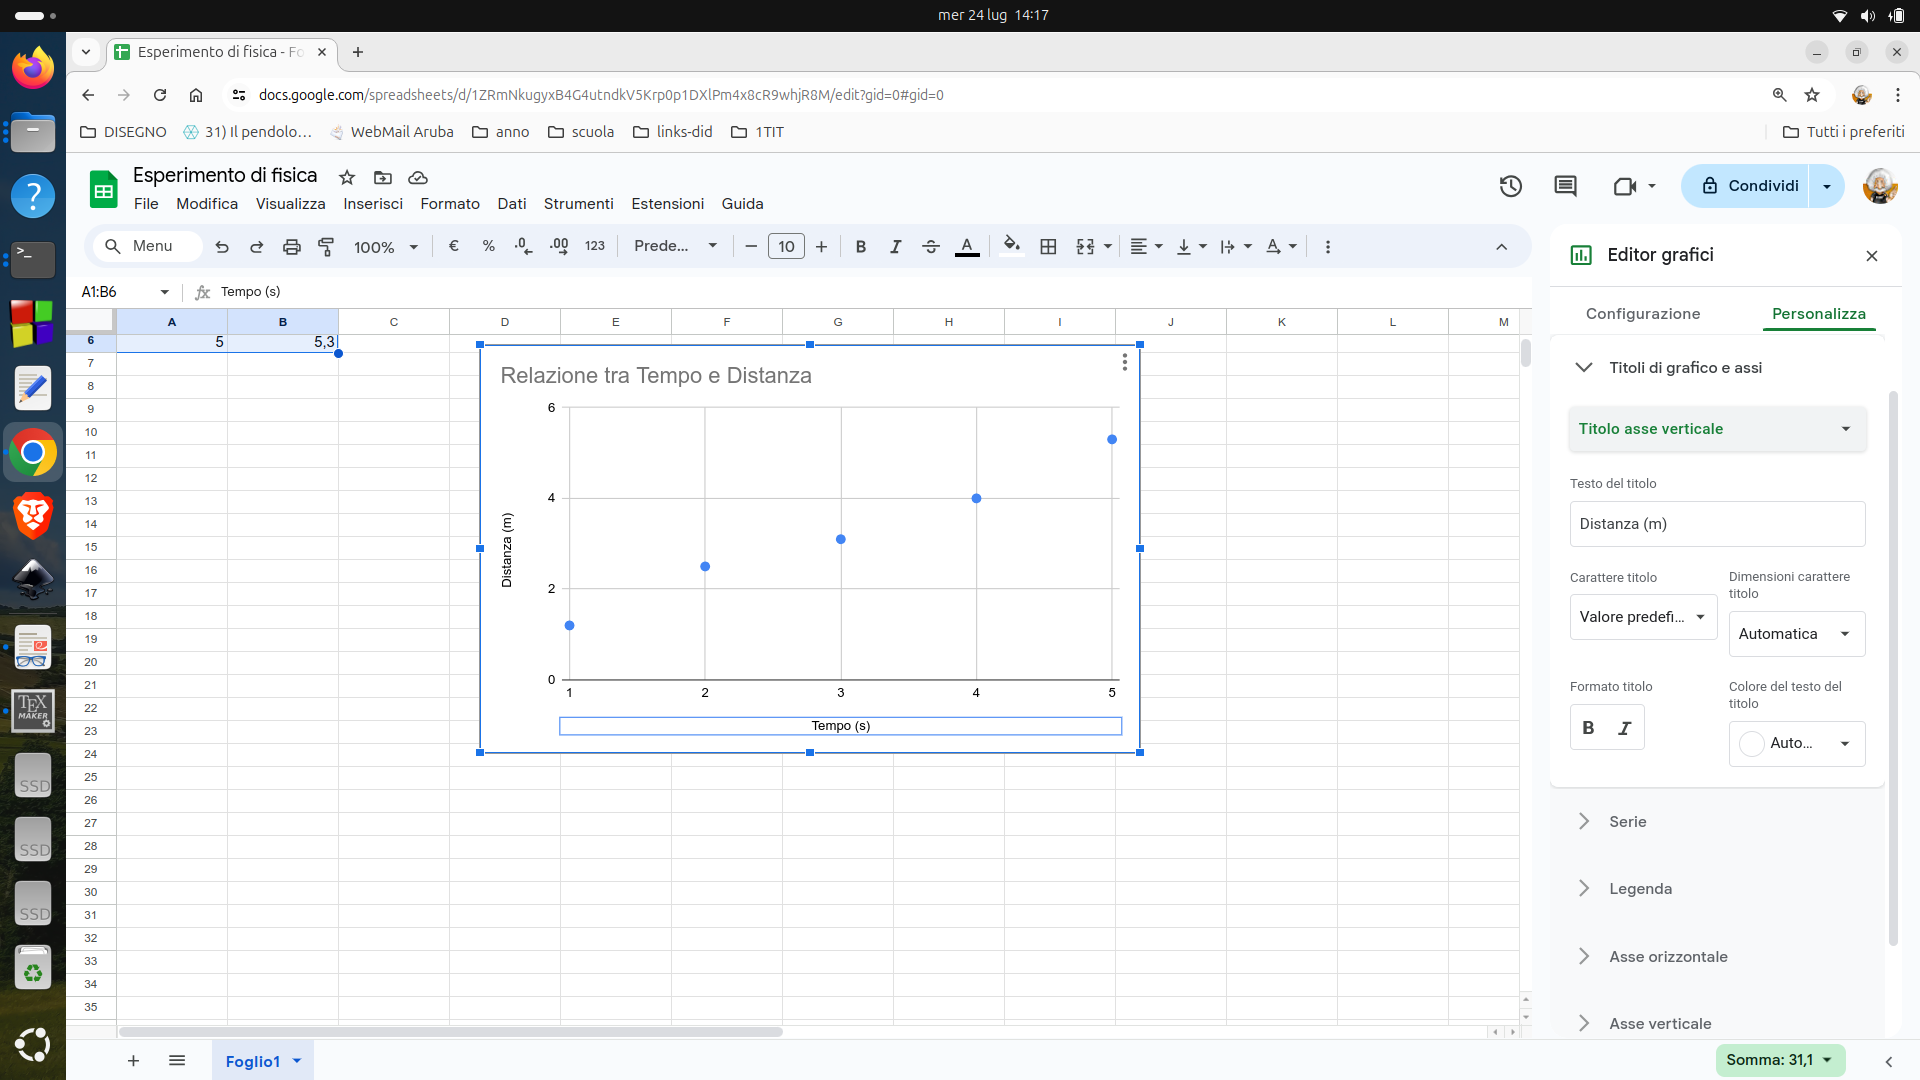
\includegraphics[width=\linewidth]{path_to_image/titoloy.png} 
    \caption{Scelta del titolo per l'asse verticale.}
    \label{fig:titoloy}
\end{figure}
        

    \item Per aggiungere una linea di tendenza, espendi il sottomenu \textbf{Serie} (figura \ref{fig:serie}) e seleziona \textbf{Linea di tendenza}. Puoi scegliere il tipo di linea di tendenza (lineare, polinomiale etc.) in base ai tuoi dati. I nostri dati sembrano adattarsi ad una retta, per cui sceglieremo \textbf{Lineare}. In fine. scegliamo di mostrare l'equazione della linea di tendenza (sottomenu \textbf{Etichetta}, voce \textbf{Utilizza equazione}. Si tratta della formula che stiamo cercando, ossia il legame tr X ed Y, figura \ref{fig:tendenza}). Anticipiamo che nel caso specifico, l'equazione mostrata è la formula che lega lo spazio al tempo in un moto rettilineo uniforme. Più avanti la scriveremo nella forma:
    \[
    s=v\cdot t +s_0
    \]
    essendo $s$ la distanza percorsa ad un certo istante $t$, $v$ la velocità costante, ed $s_0$ la posizione iniziale del moto. Possiamo vedere che il corpo si è mosso ad una velocità di $\SI{0,97}{\meter\per\second}$ partendo da una posizione all'istante zero pari a $\SI{0,31}{\meter}$. Perché è comoda questa equazione? L'equazione permette di calcolare la posizione ad un qualunque istante, anche se non presente in tabella. Ad esempio, per $t=\SI{2,9}{\second}$, abbiamo:
    
    \[
    s=\left(\SI{0,97}{\meter\per\second}\right)\times \left( \SI{2,9}{\second}\right) + \SI{0,31}{\meter}=\SI{3,12}{\meter}.
    \]
    
\begin{figure}[h!]
    \centering
    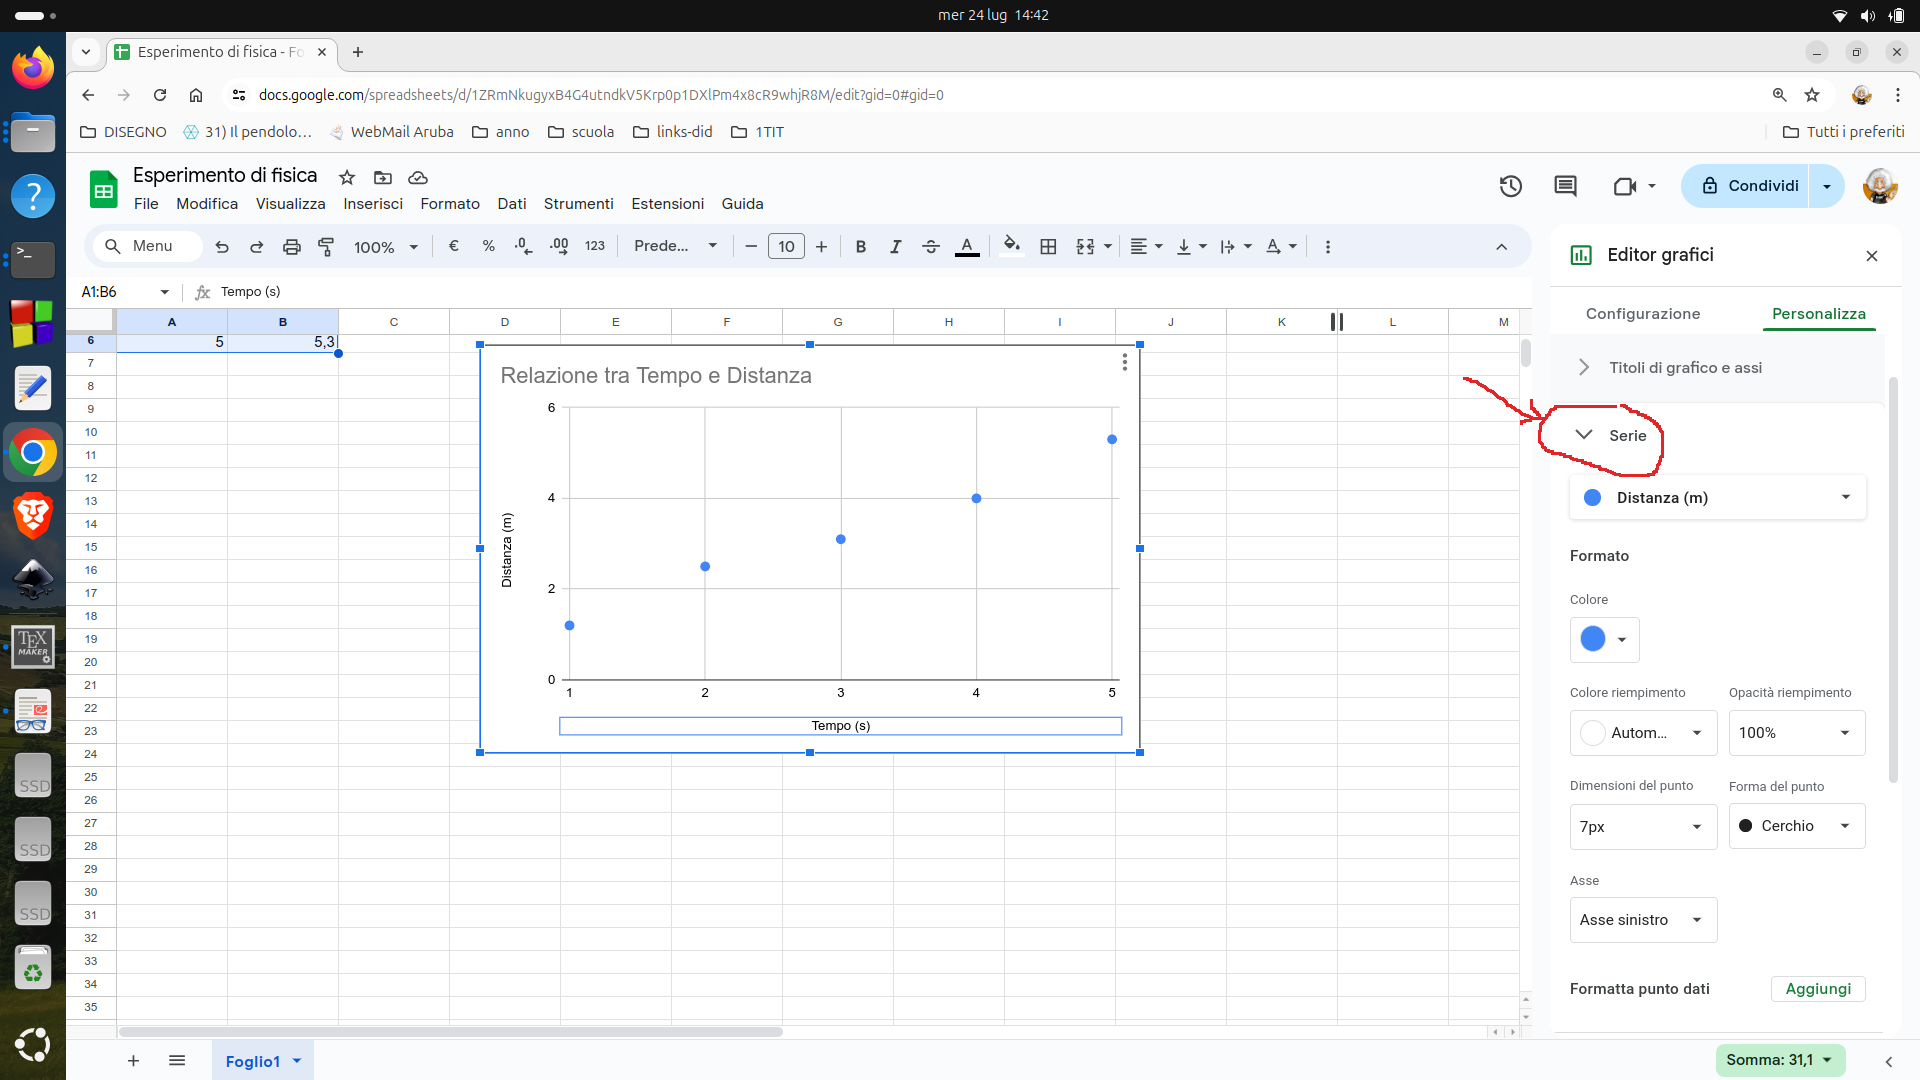
\includegraphics[width=\linewidth]{path_to_image/serie.png} 
    \caption{Scheda \textbf{serie} per la linea di tendenza.}
    \label{fig:serie}
\end{figure}    
  \begin{figure}[h!]
    \centering
    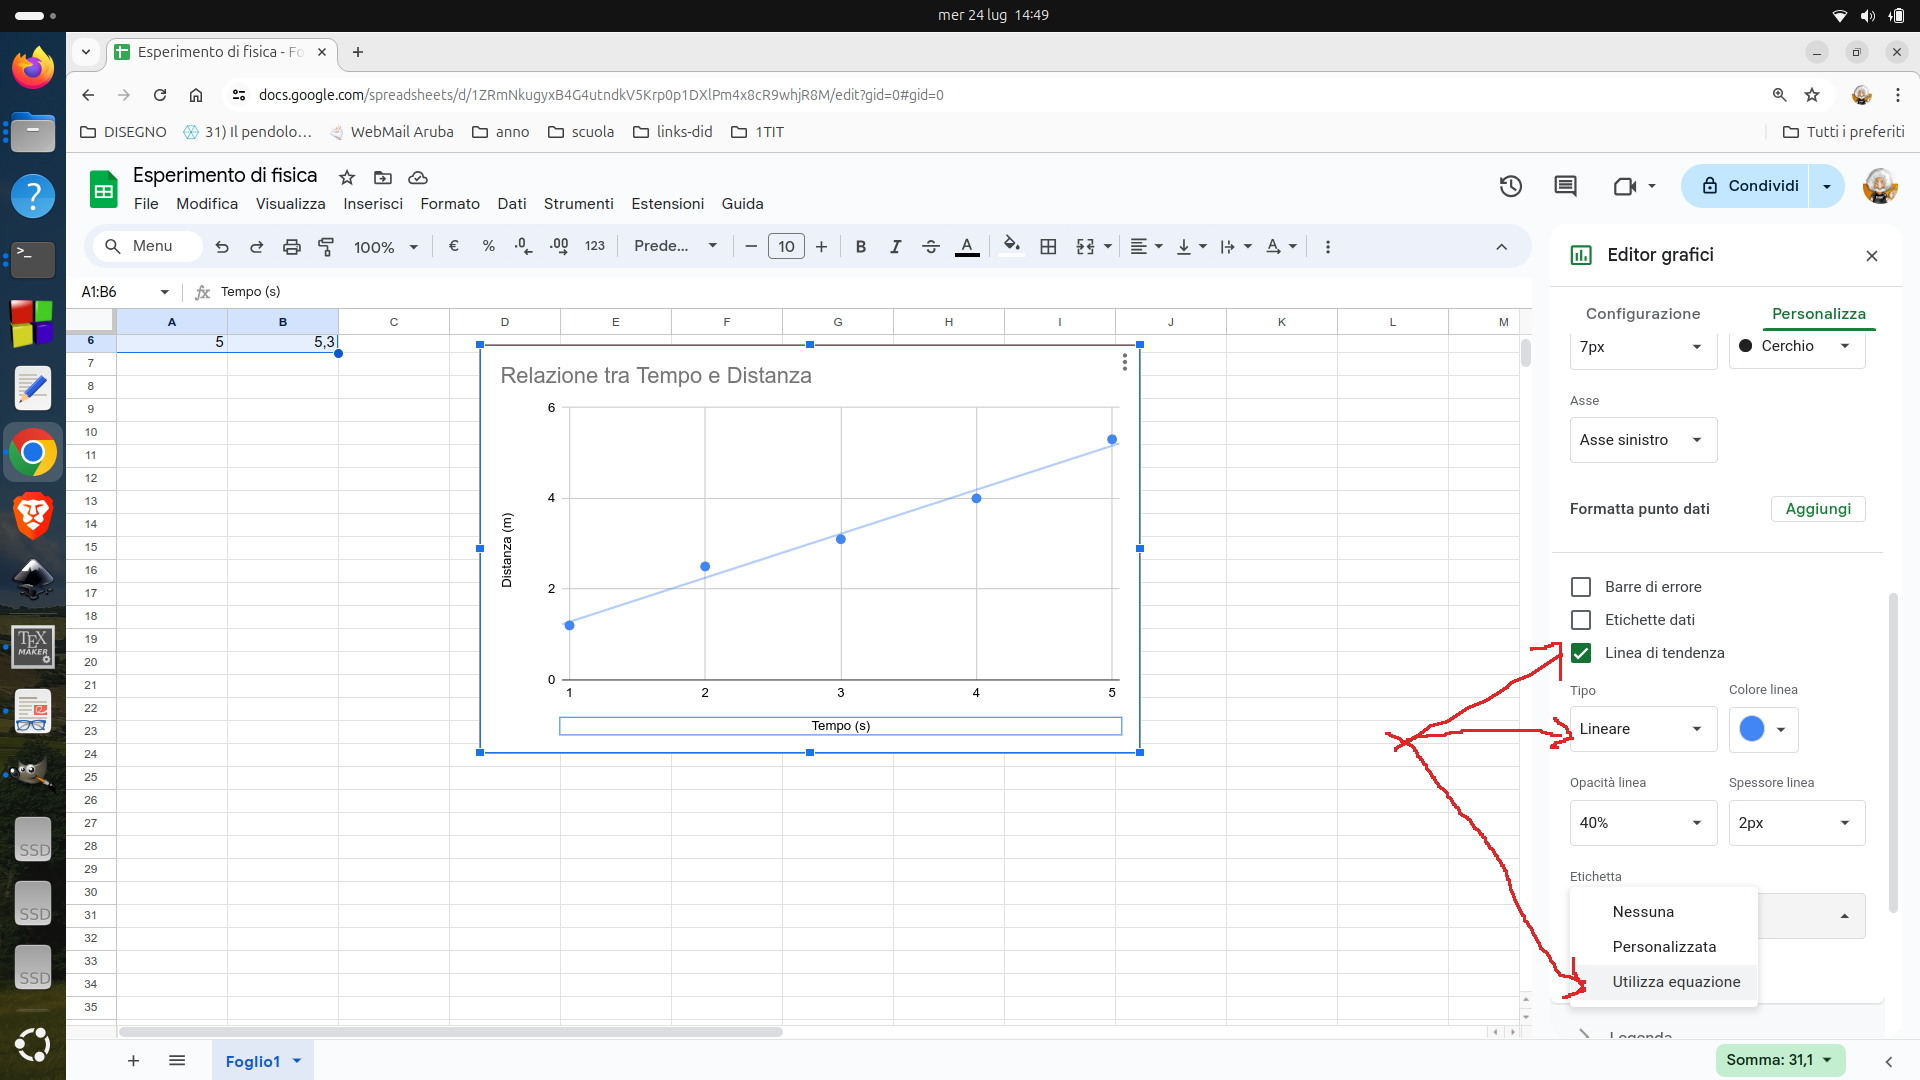
\includegraphics[width=\linewidth]{path_to_image/tendenza.png} 
    \caption{Scheda \textbf{serie} Inserimento linea di tendenza lineare (retta).}
    \label{fig:tendenza}
\end{figure}    
   In generale non è facile scegliere il tipo di linea di tendenza. In fisica, i dati possono essere legati da una relazione di proporzionalità diretta, quadratica, inversa, quadratica inversa o molte altre. Il tipo lineare è il più semplice. Quando i grafici hanno un andamento curvo, è possibile che i dati siano legati da una formula parabolica (ossia una formula del tipo $y=ax^2 +bx +c$.) In questo caso, la linea di tendenza sarà una parabola. Nei fogli google, basterà selezionare dal sottomenu la linea \textbf{Polinomiale} (figura \ref{fig:polinomiale}):
   \begin{figure}[h!]
    \centering
    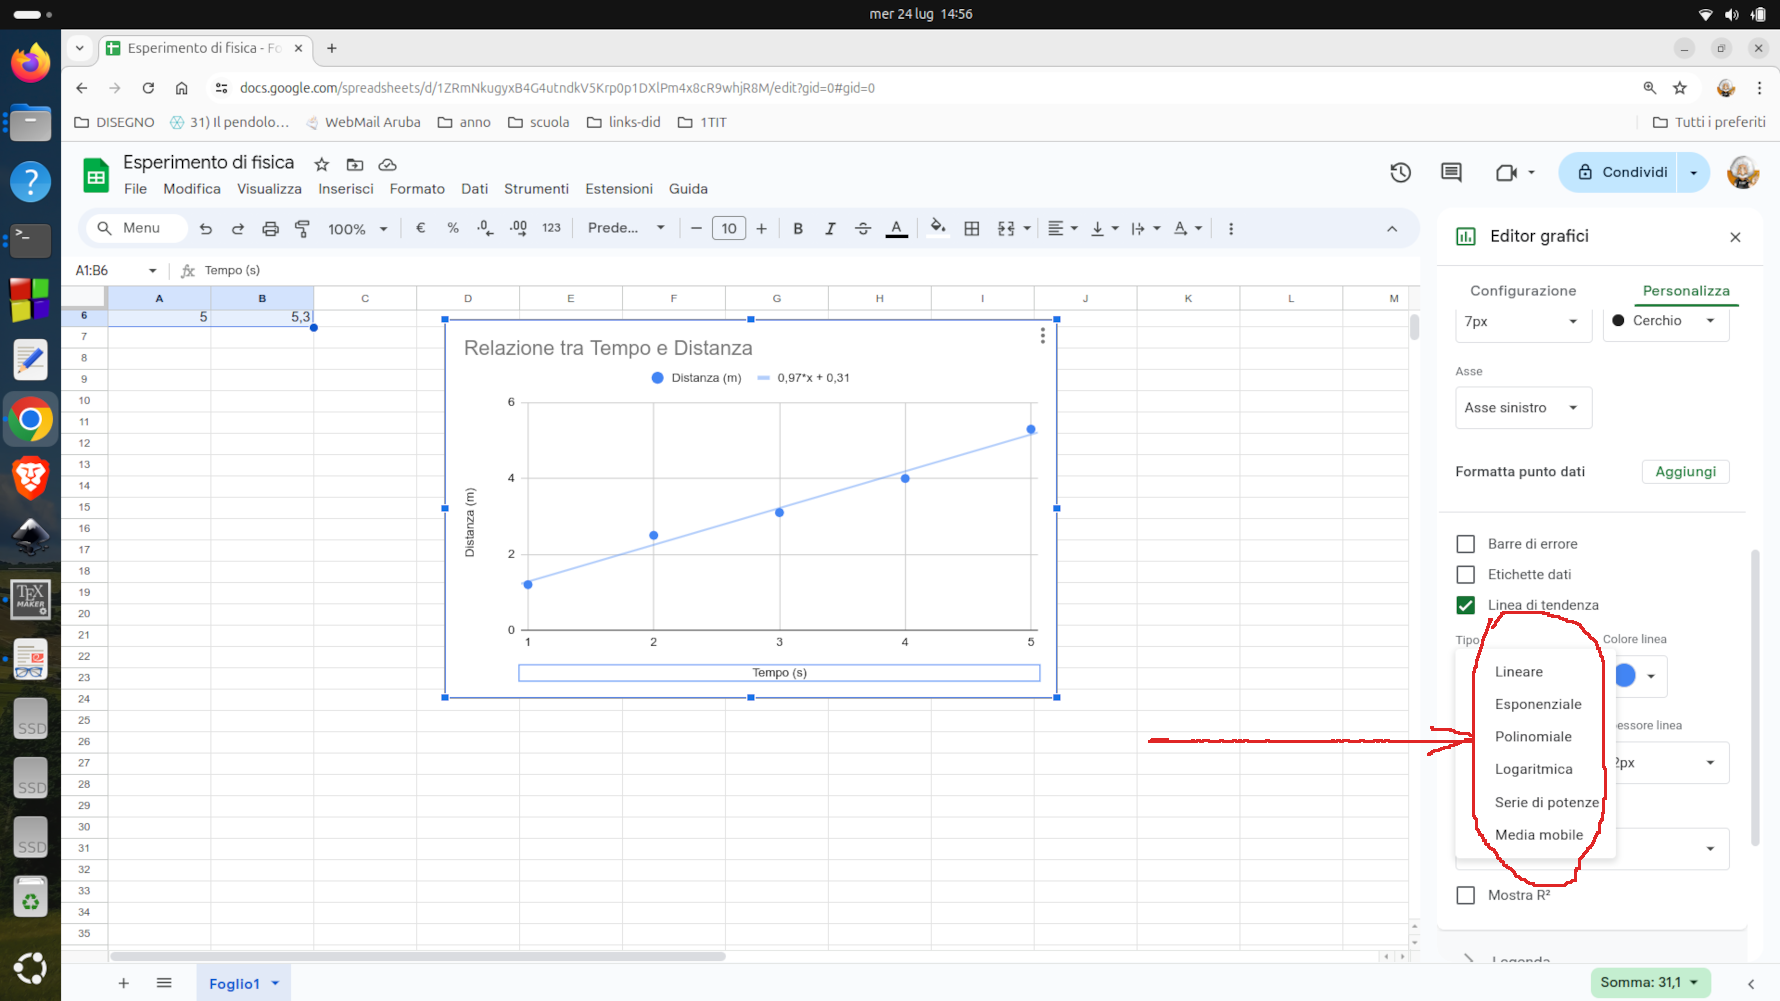
\includegraphics[width=\linewidth]{path_to_image/polinomiale.png} 
    \caption{Scelta per l'inserimento della linea di tendenza polinomiale (parabola).}
    \label{fig:polinomiale}
\end{figure}     
 In generale, ti consiglio di provare varie linee di tendenza, in modo da trovare quella che meglio si adatta ai dati.    L'adattamento è tanto migliore quanto più il cosiddetto fatto $R^2$ è vicino ad uno. Per visualizzare questo fattore sul grafico, barrare la casella $\mathbf{Mostra \,\,R^2}$ come in figura \ref{fig:r2}:
 
   \begin{figure}[h!]
    \centering
    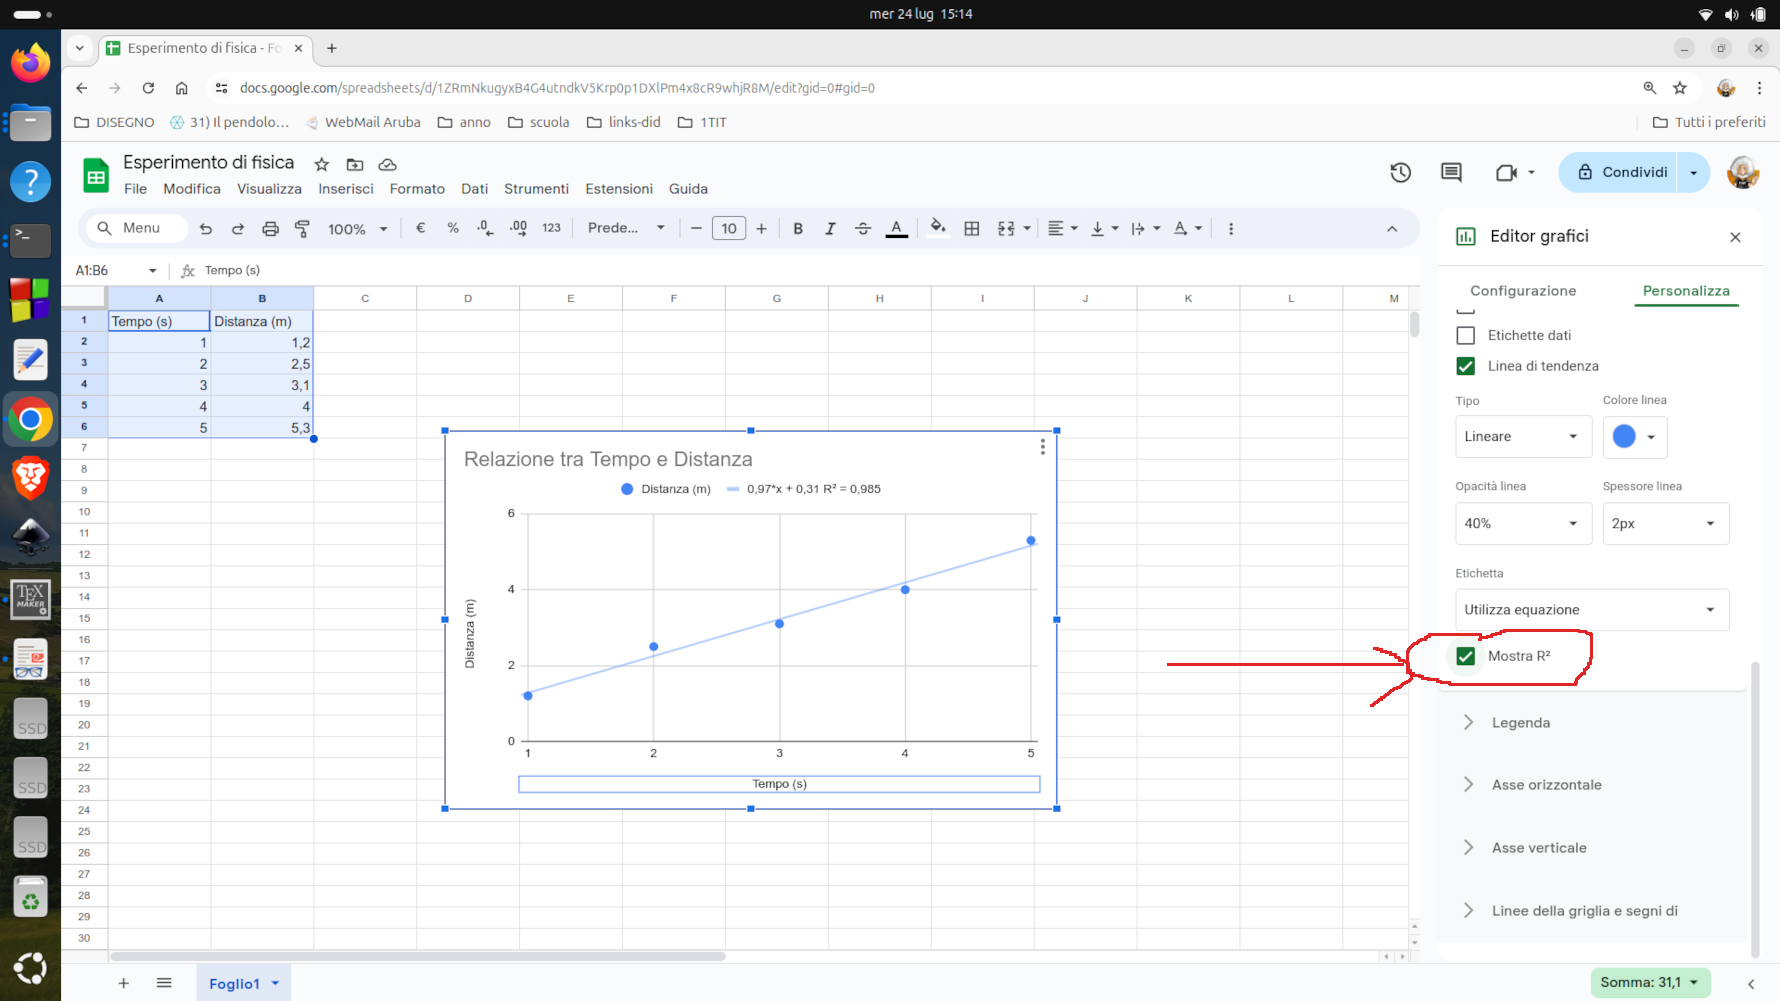
\includegraphics[width=\linewidth]{path_to_image/r2.png} 
    \caption{Visualizzazione del parametro $R^2$.}
    \label{fig:r2}
 \end{figure}
 
    
\end{enumerate}
Tutti gli elementi grafici e  testuali sono ulteriormente personalizzabili (ad esempio l'aspetto dei punti del grafico, il font per i titoli degli assi etc.). Ti consiglio di sperimentare con questi aspetti modificando a tuo piacimemnto questi elementi dalla scheda personalizzazione. Il loro uso è molto intuitivo.

\section{Visualizzare Due Grafici Contemporaneamente}
\begin{enumerate}
    \item Inserisci una nuova serie di dati in una colonna diversa. Ad esempio, nella colonna C metti i valori della variabile dipendente di un secondo esperimento (ad esempio, distanza in metri).
    \item Esempio di dati:
    \begin{center}
    \begin{tabular}{|c|c|c|}
    \hline
    Tempo (s) & Distanza 1 (m) & Distanza 2 (m) \\
    \hline
    1 & 1,2 & 0,8 \\
    2 & 2,5 & 1,5 \\
    3 & 3,1 & 2,2 \\
    4 & 4,0 & 3,0 \\
    5 & 5,3 & 4,1 \\
    \hline
    \end{tabular}
    \end{center}
    \item Seleziona i dati inseriti nelle colonne A, B e C. Puoi farlo cliccando e trascinando il mouse dall'angolo superiore sinistro (A1) all'angolo inferiore destro (C5) dei tuoi dati oppure (vedi figura \ref{fig:intervallo2}) selezionando \textbf{aggiungi serie}, figura \ref{fig:intervallo2} e. successivamente, cliccando il tasto ``+''. Si aprirà un campo di testo in cui inserire l'intervallo di cella. Per farlo, si può agire graficamente, selezionando tutta la colonna col tasto destro del mouse e verrà automaticamente scritto l'intervallo (figura \ref{fig:intervallo2-dialogo}la scrittura \textit{Foglio1!C1:C6} indica di selezionare l'intervallo del foglio attuale (Foglio1) dalla cella C1 alla cella C6). In fine clicca ``Ok'' e la serie verrà oinserita. A quesato punto puoi personalizzare il grafico come vuoi, inserire linee di tendenza etc. Come regola generale, si consiglia di realizzare grafici in cui le due serie sullì'asse Y sono della stessa natura ma non è vietato inserire anche serie diverse purché, è bene ribadirlo, sull'asse X, deve esserci una sola serie (nel nostro caso, il tempo). Come esercizio, puoi provare a disegnare la linea di tendenza della serie 2. Il grafico finale è in figura \ref{fig:finale}.
    
      \begin{figure}[h!]
    \centering
    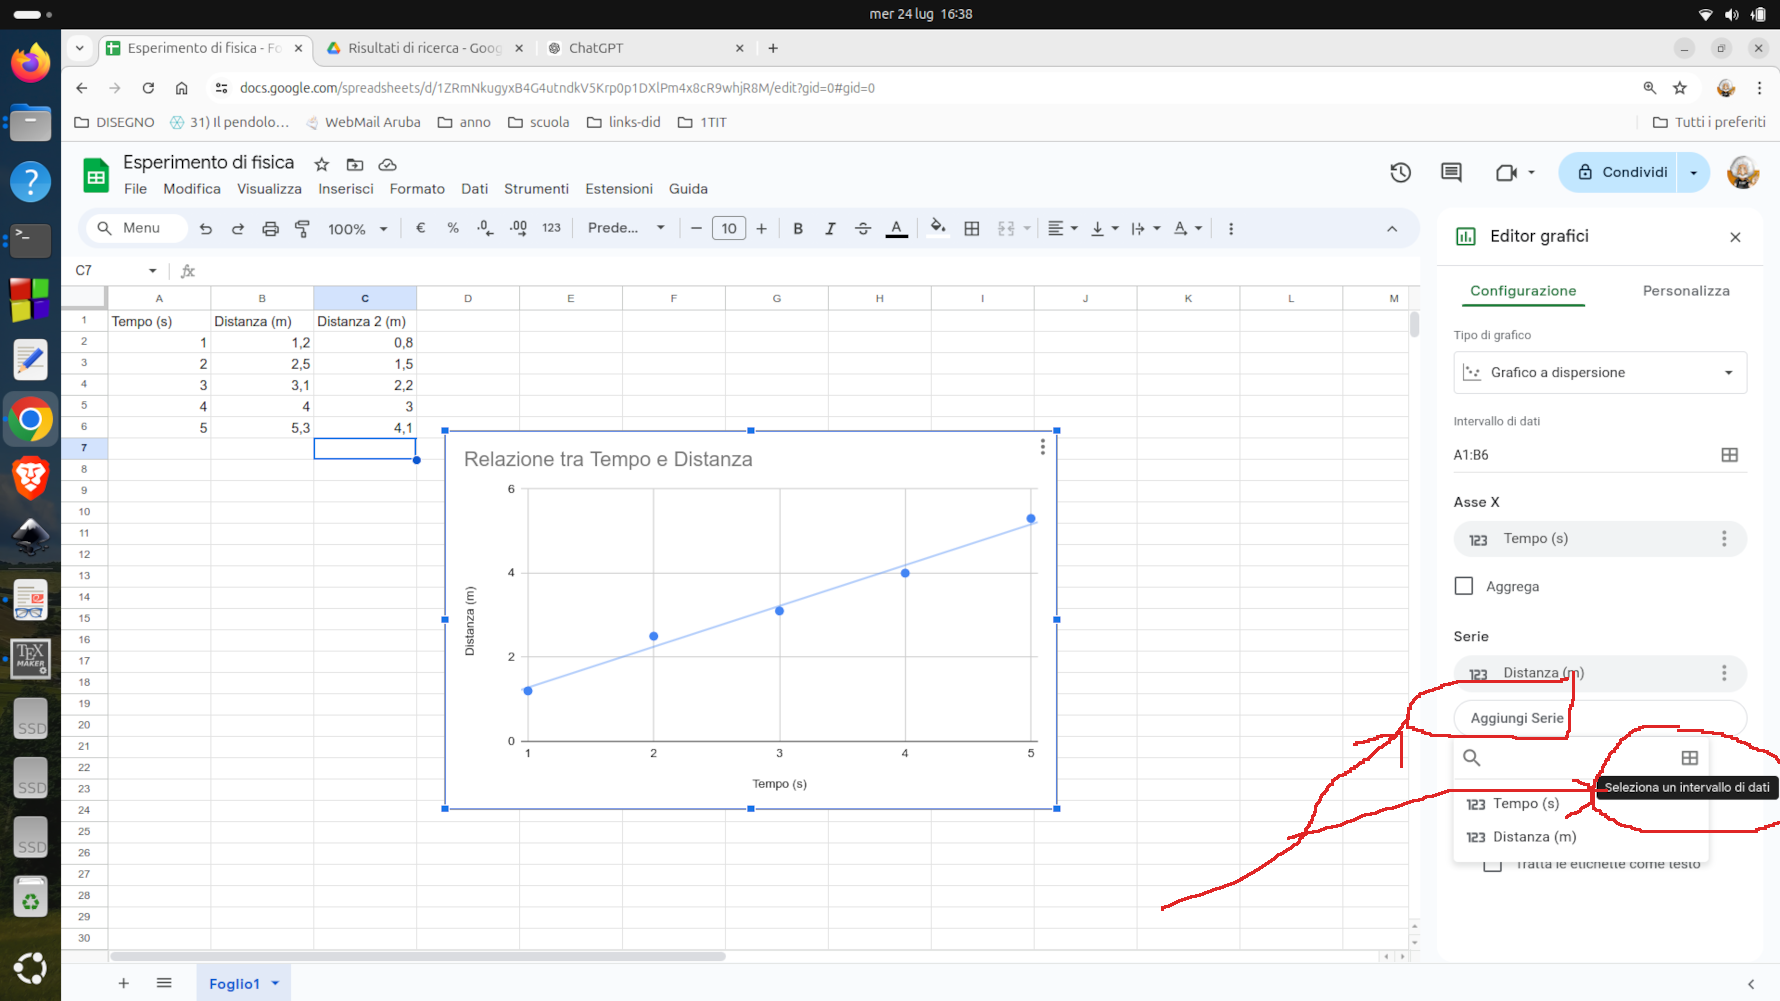
\includegraphics[width=\linewidth]{path_to_image/intervallo2.png} 
    \caption{Selezione di una serie, tasto ``+''.}
    \label{fig:intervallo2}
 \end{figure} 
    
    
\begin{figure}[h!]
    \centering
    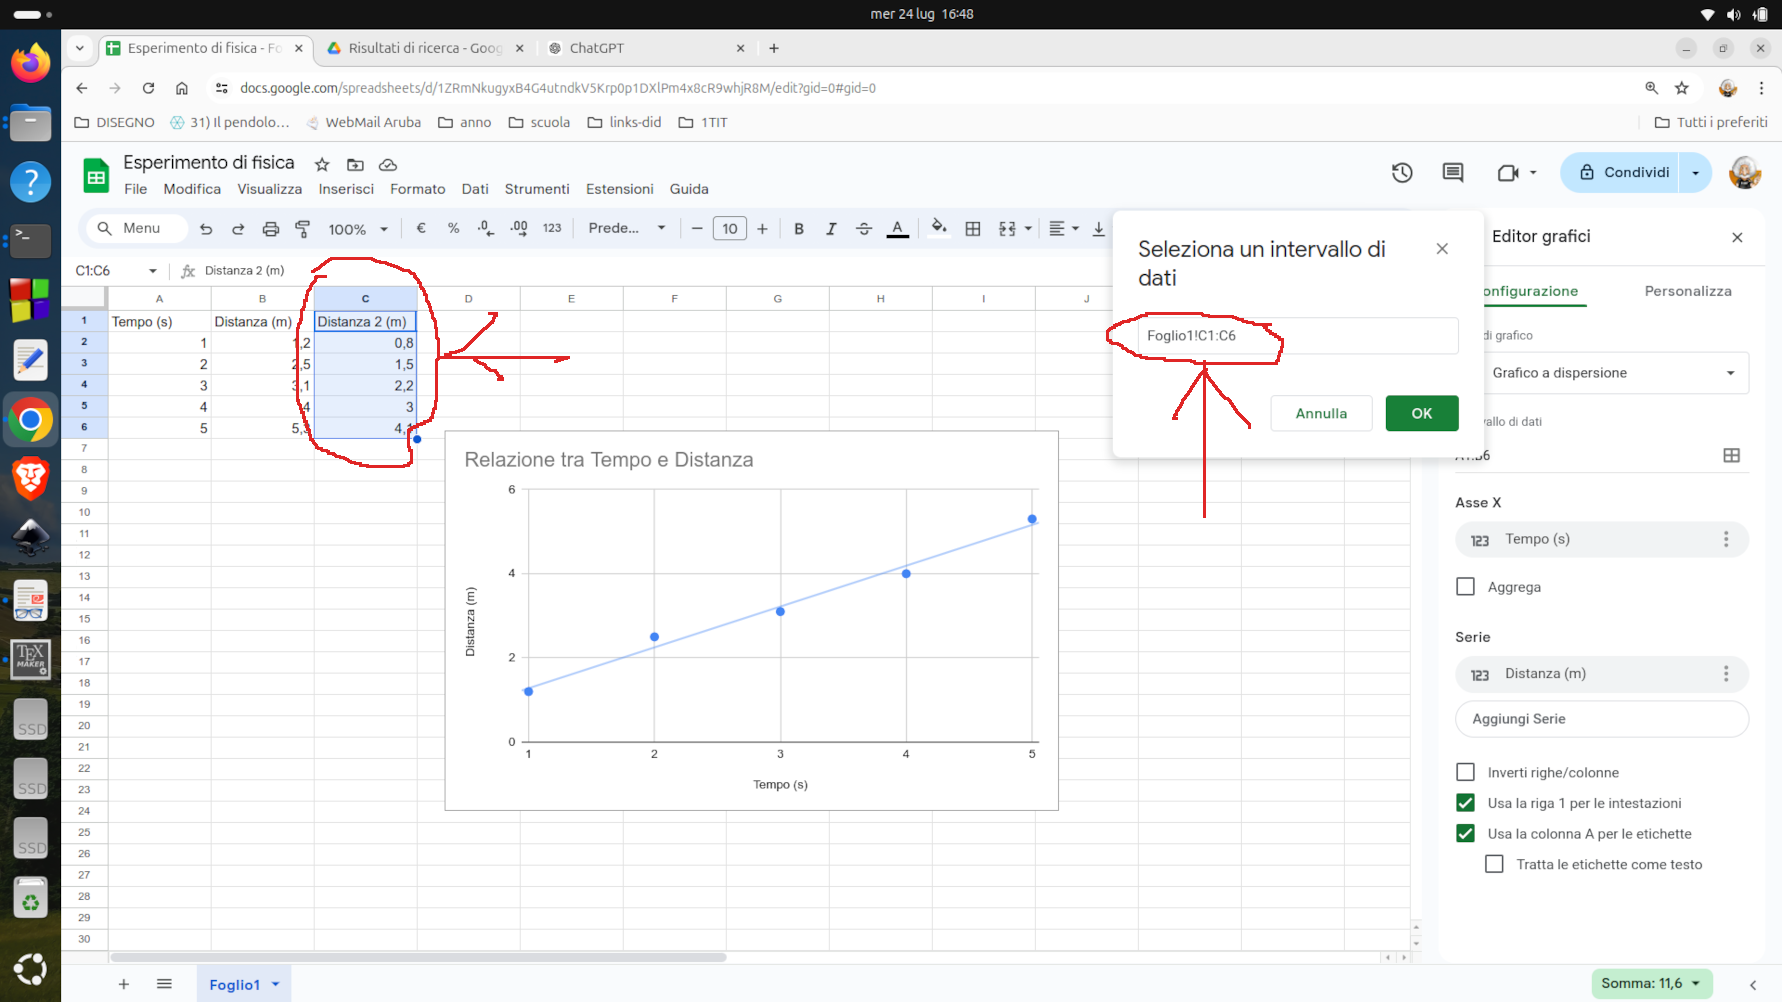
\includegraphics[width=\linewidth]{path_to_image/intervallo2-dialogo.png} 
    \caption{Finestra di dialogo per la scelta dell'intervallo della serie 2.}
    \label{fig:intervallo2-dialogo}
 \end{figure} 

\begin{figure}[h!]
    \centering
    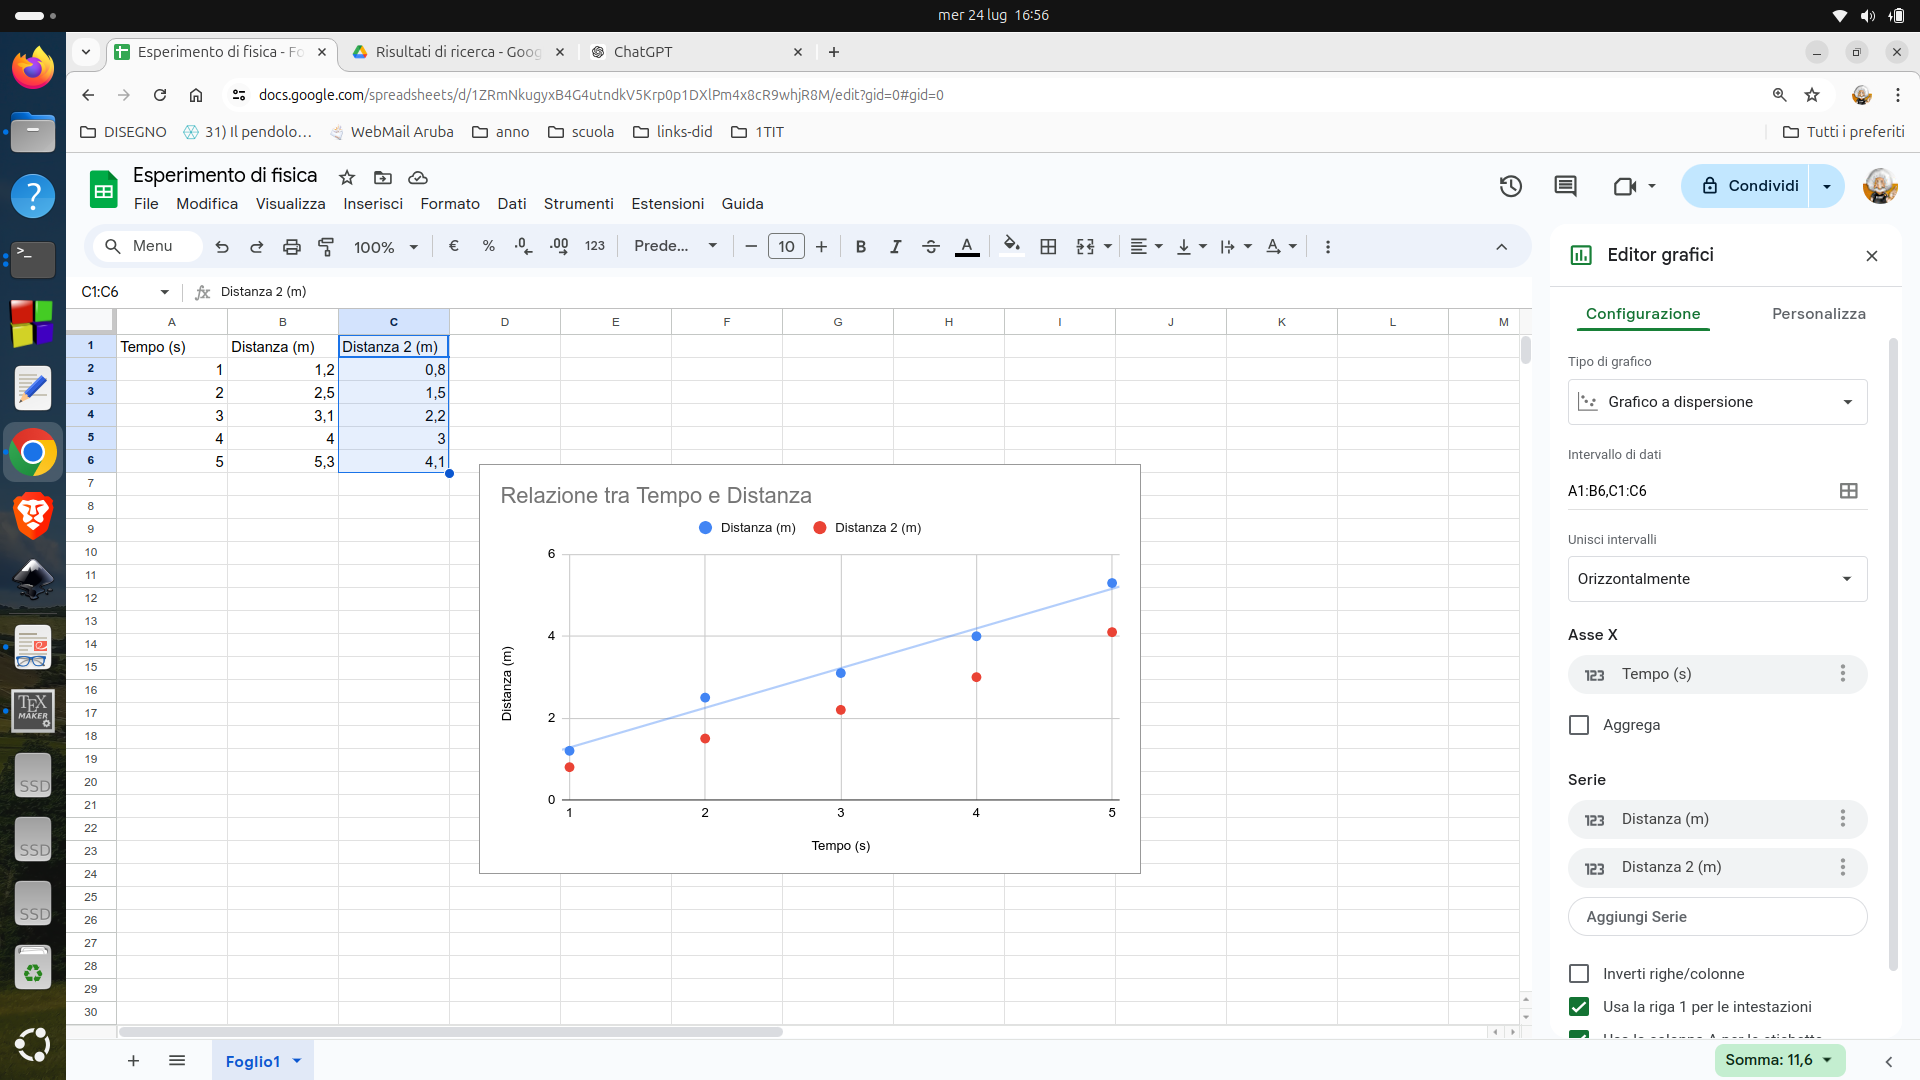
\includegraphics[width=\linewidth]{path_to_image/finale.png} 
    \caption{COme si presenta il grafico costruito nel tutorial.}
    \label{fig:finale}
 \end{figure} 
\end{enumerate}

\section{Conclusione}
Seguendo questi passaggi, sarai in grado di creare e personalizzare grafici a dispersione su Google Sheets per analizzare e visualizzare i tuoi dati sperimentali. Questa competenza è utile non solo per le lezioni di fisica, ma anche per altre discipline scientifiche.

\end{document}
